%Lampiran merupakan data atau pelengkap atau hasil olahan yang menunjang penulisan tugas akhir, tetapi tidak dicantumkan di dalam isi tugas akhir, karena akan mengganggu kesinambungan pembacaan. Lampiran yang perlu disertakan dikelompokkan menurut jenisnya, antara lain jadwal, tabel, daftar pertanyaan, gambar, grafik, desain. Pengelompokan lampiran disesuaikan dengan kebijakan fakultas.

%Ketentuan pembuatan lampiran adalah sebagai berikut.
%a. Nomor dan judul lampiran ditulis di sudut kanan atas halaman (right-aligned) dengan huruf tegak tipe Times New Roman 12 poin.
%b. Judul lampiran ditik dalam satu baris menggunakan huruf kapital di awal kata (titlecase).
%c. Lampiran yang lebih dari satu halaman, pada halaman berikutnya diberi keterangan ?lanjutan? dalam tanda kurung pada sudut kanan atas halaman (right-aligned).
%d. Isi dan urutan pengelompokan lampiran disesuaikan dengan kebijakan fakultas


%-----------------------------------------------------------------------------%
\addChapter{Contoh bank pohon struktur dependensi ragam tulis}
\chapter*{Lampiran 1: Contoh Bank Pohon Struktur Dependensi Ragam Tulis}
%-----------------------------------------------------------------------------%

\begin{figure}
	\centering 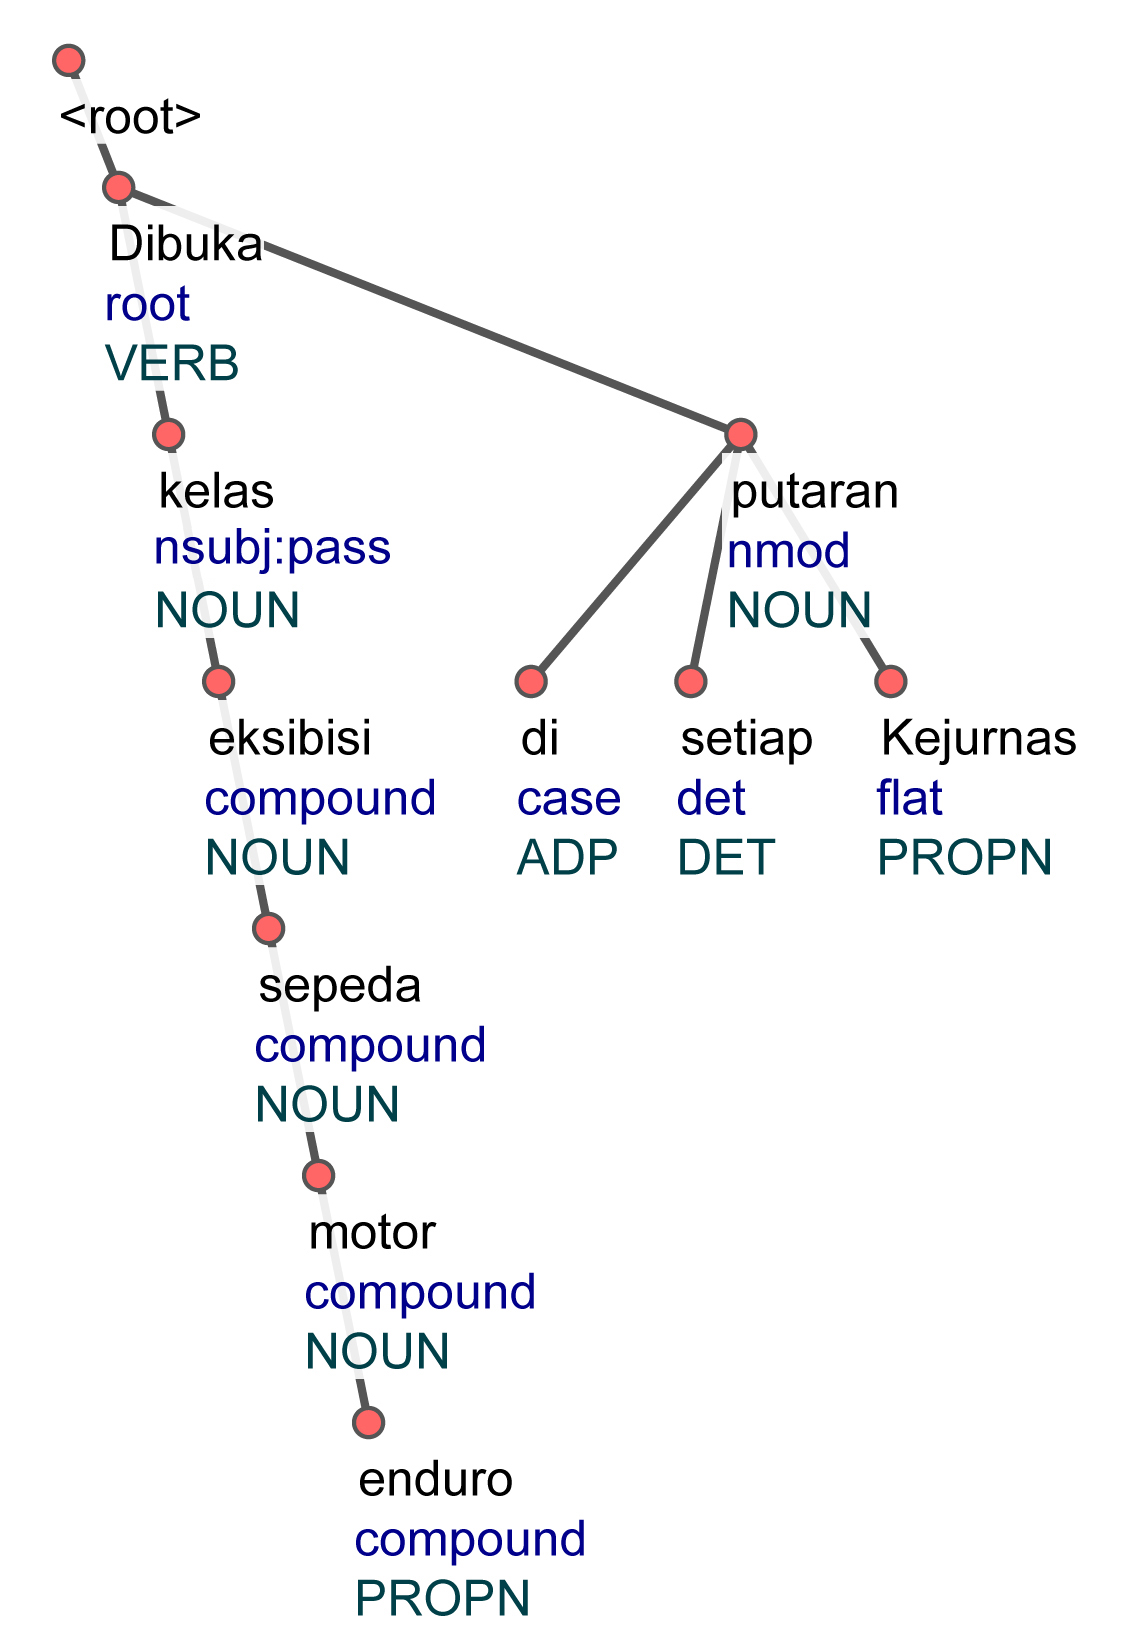
\includegraphics[width=0.35
	\textwidth] {pics/lampiran/lampirants770.jpg} 
	\caption{Bank pohon struktur dependensi ragam tulis dokumen 770} 
	\label{fig:lampirants770} 
\end{figure}

\begin{figure}
	\centering 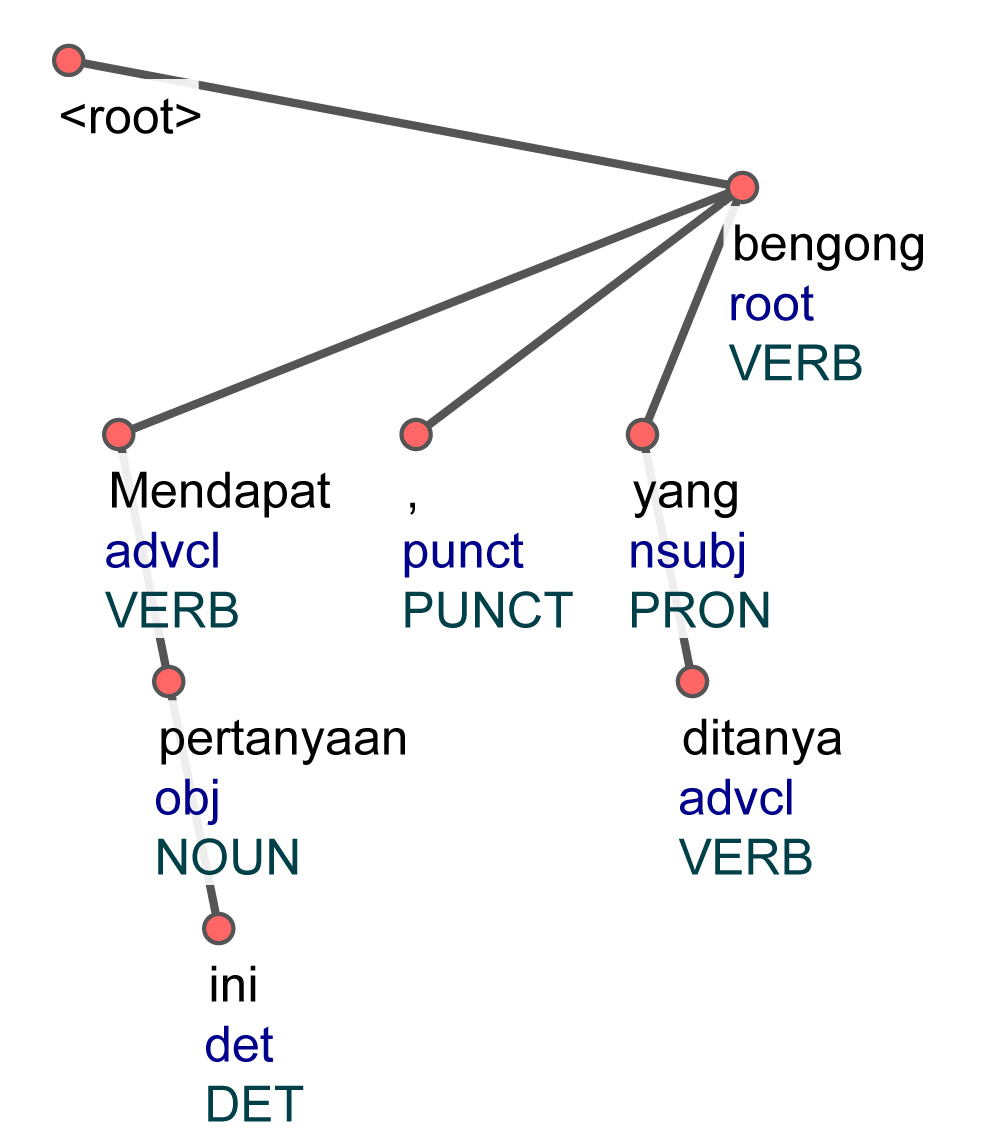
\includegraphics[width=0.3
	\textwidth] {pics/lampiran/lampirants1956.jpg} 
	\caption{Bank pohon struktur dependensi ragam tulis dokumen 1956} 
	\label{fig:lampirants1956} 
\end{figure}

\begin{figure}
	\centering 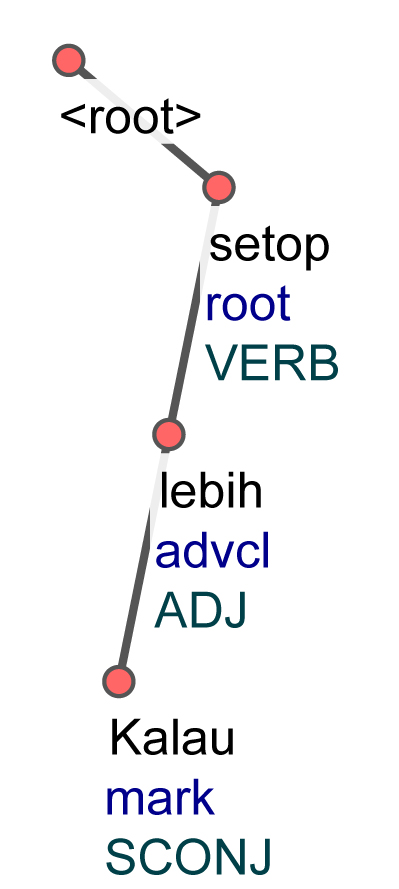
\includegraphics[width=0.15
	\textwidth] {pics/lampiran/lampirants2537.jpg} 
	\caption{Bank pohon struktur dependensi ragam tulis dokumen 2537} 
	\label{fig:lampirants2537} 
\end{figure}

\begin{figure}
	\centering 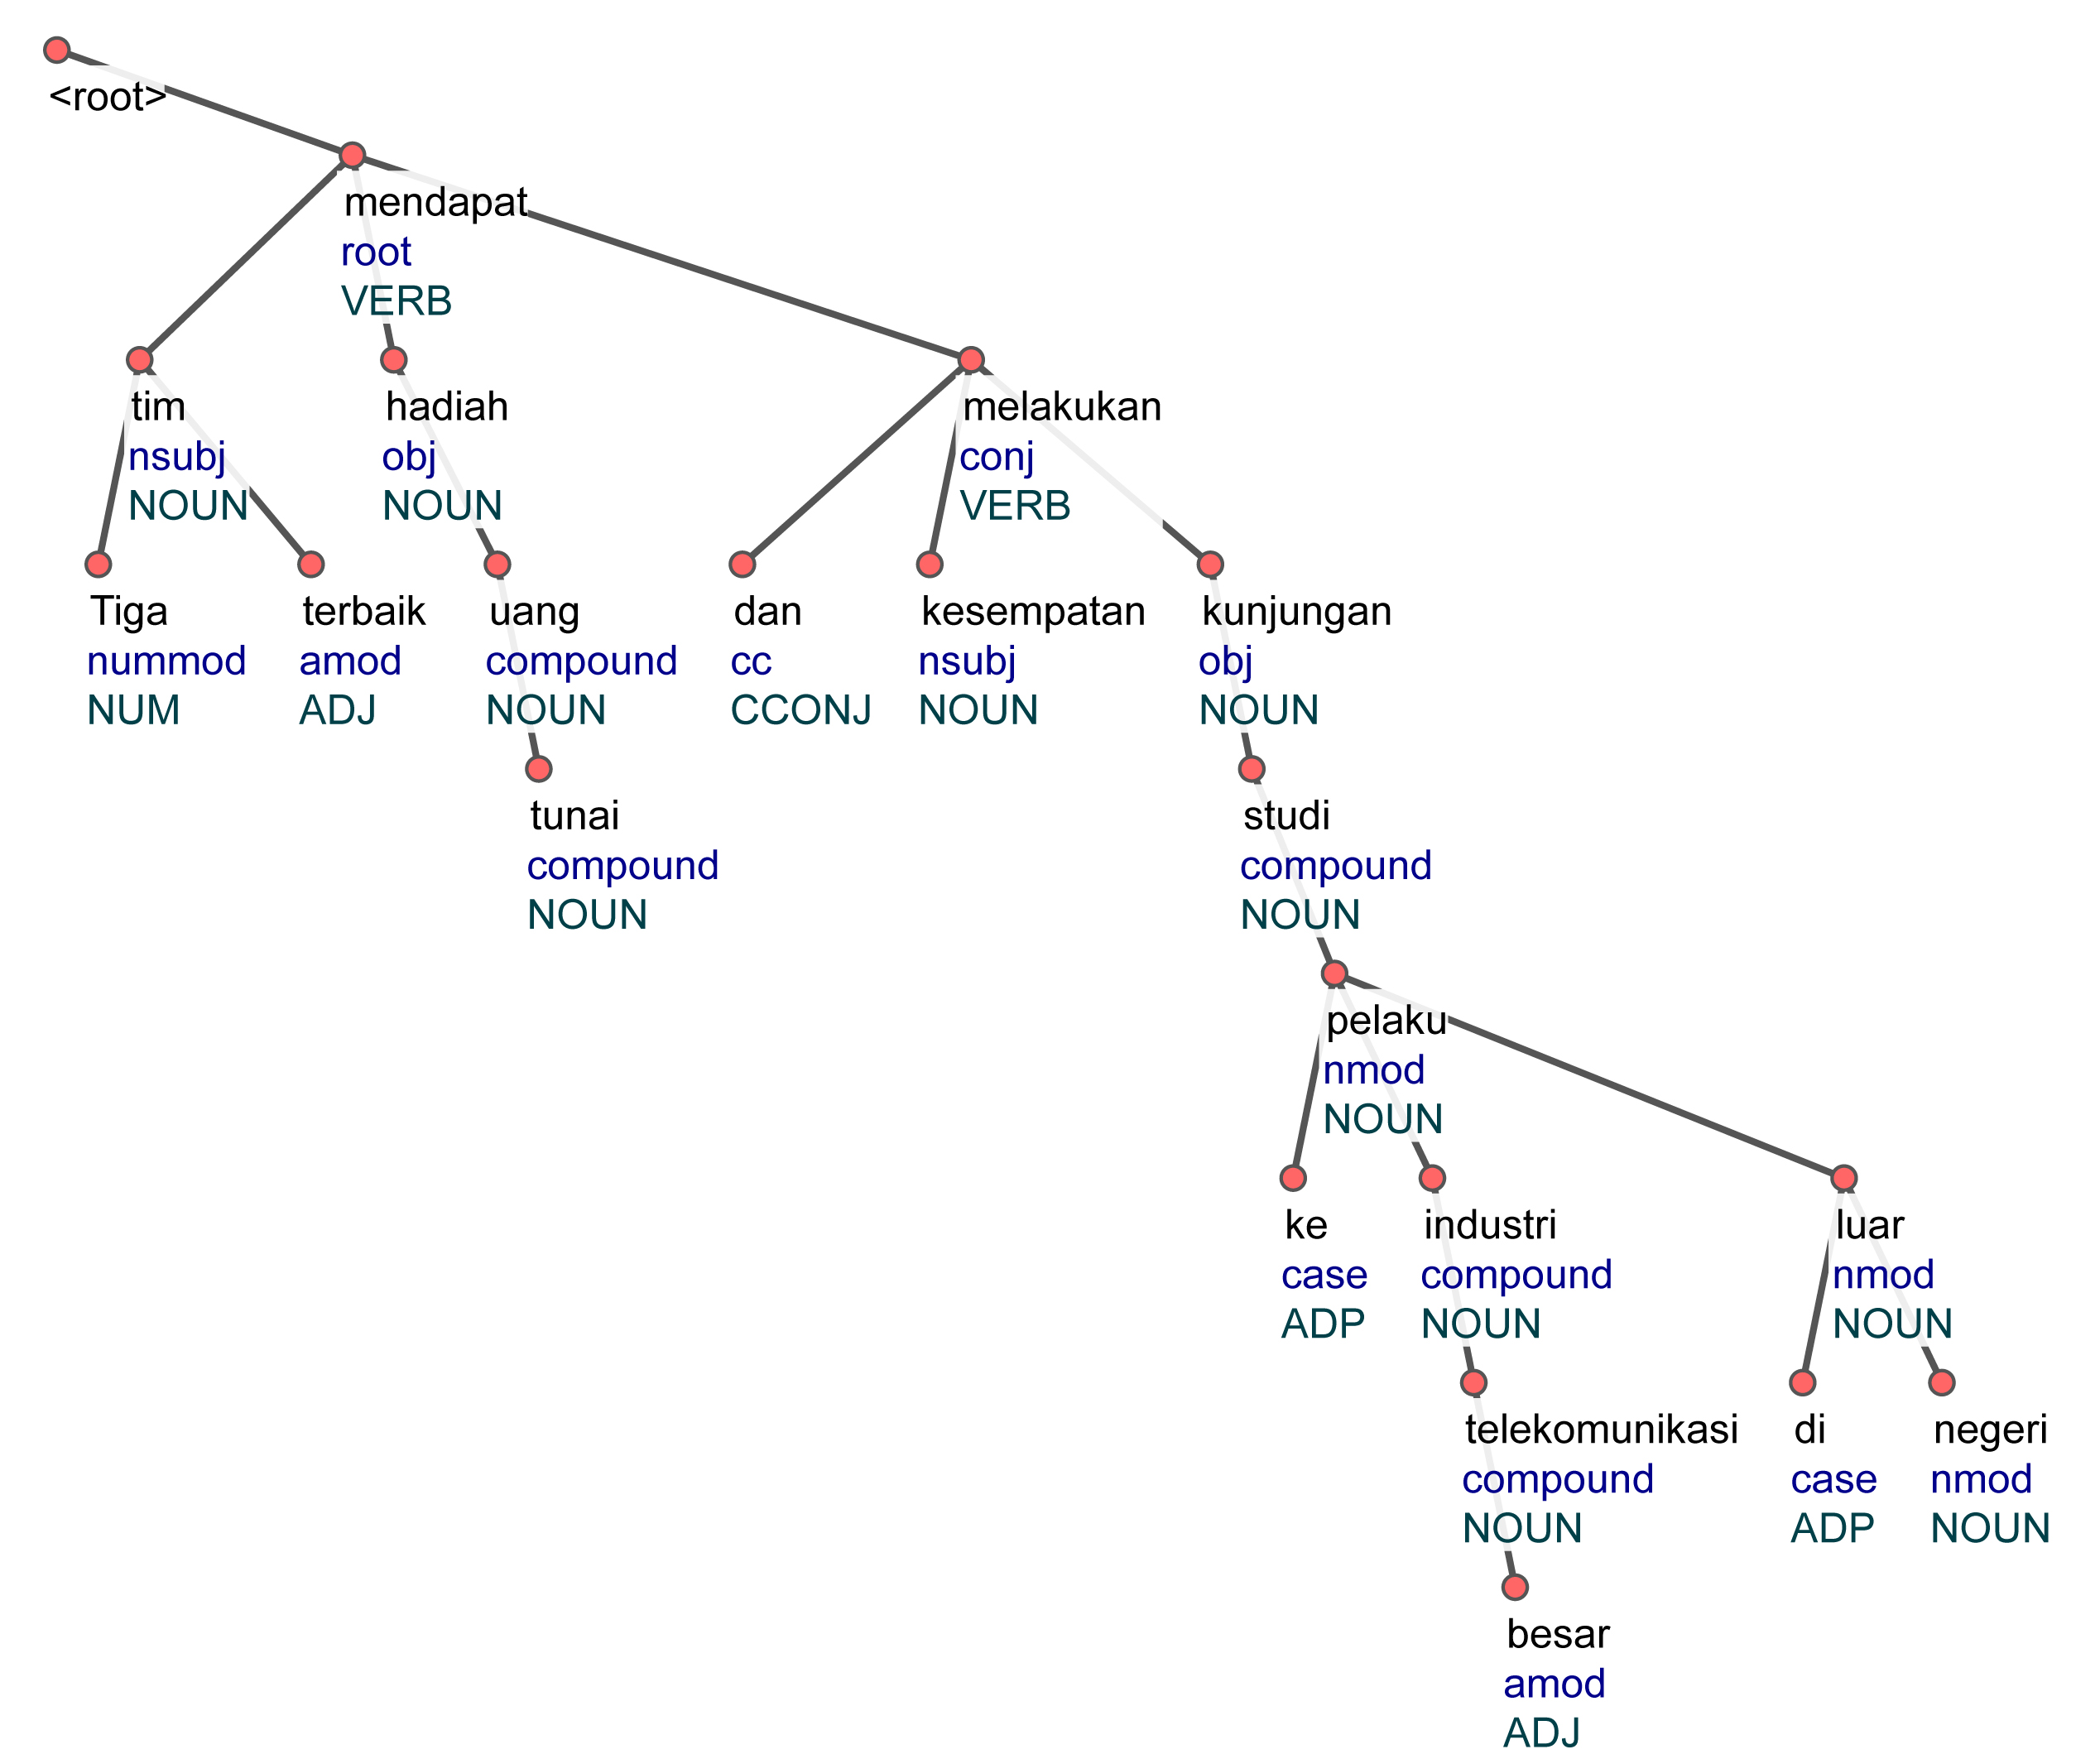
\includegraphics[width=0.8
	\textwidth] {pics/lampiran/lampirants2624.jpg} 
	\caption{Bank pohon struktur dependensi ragam tulis dokumen 2624} 
	\label{fig:lampirants2624} 
\end{figure}

\begin{figure}
	\centering 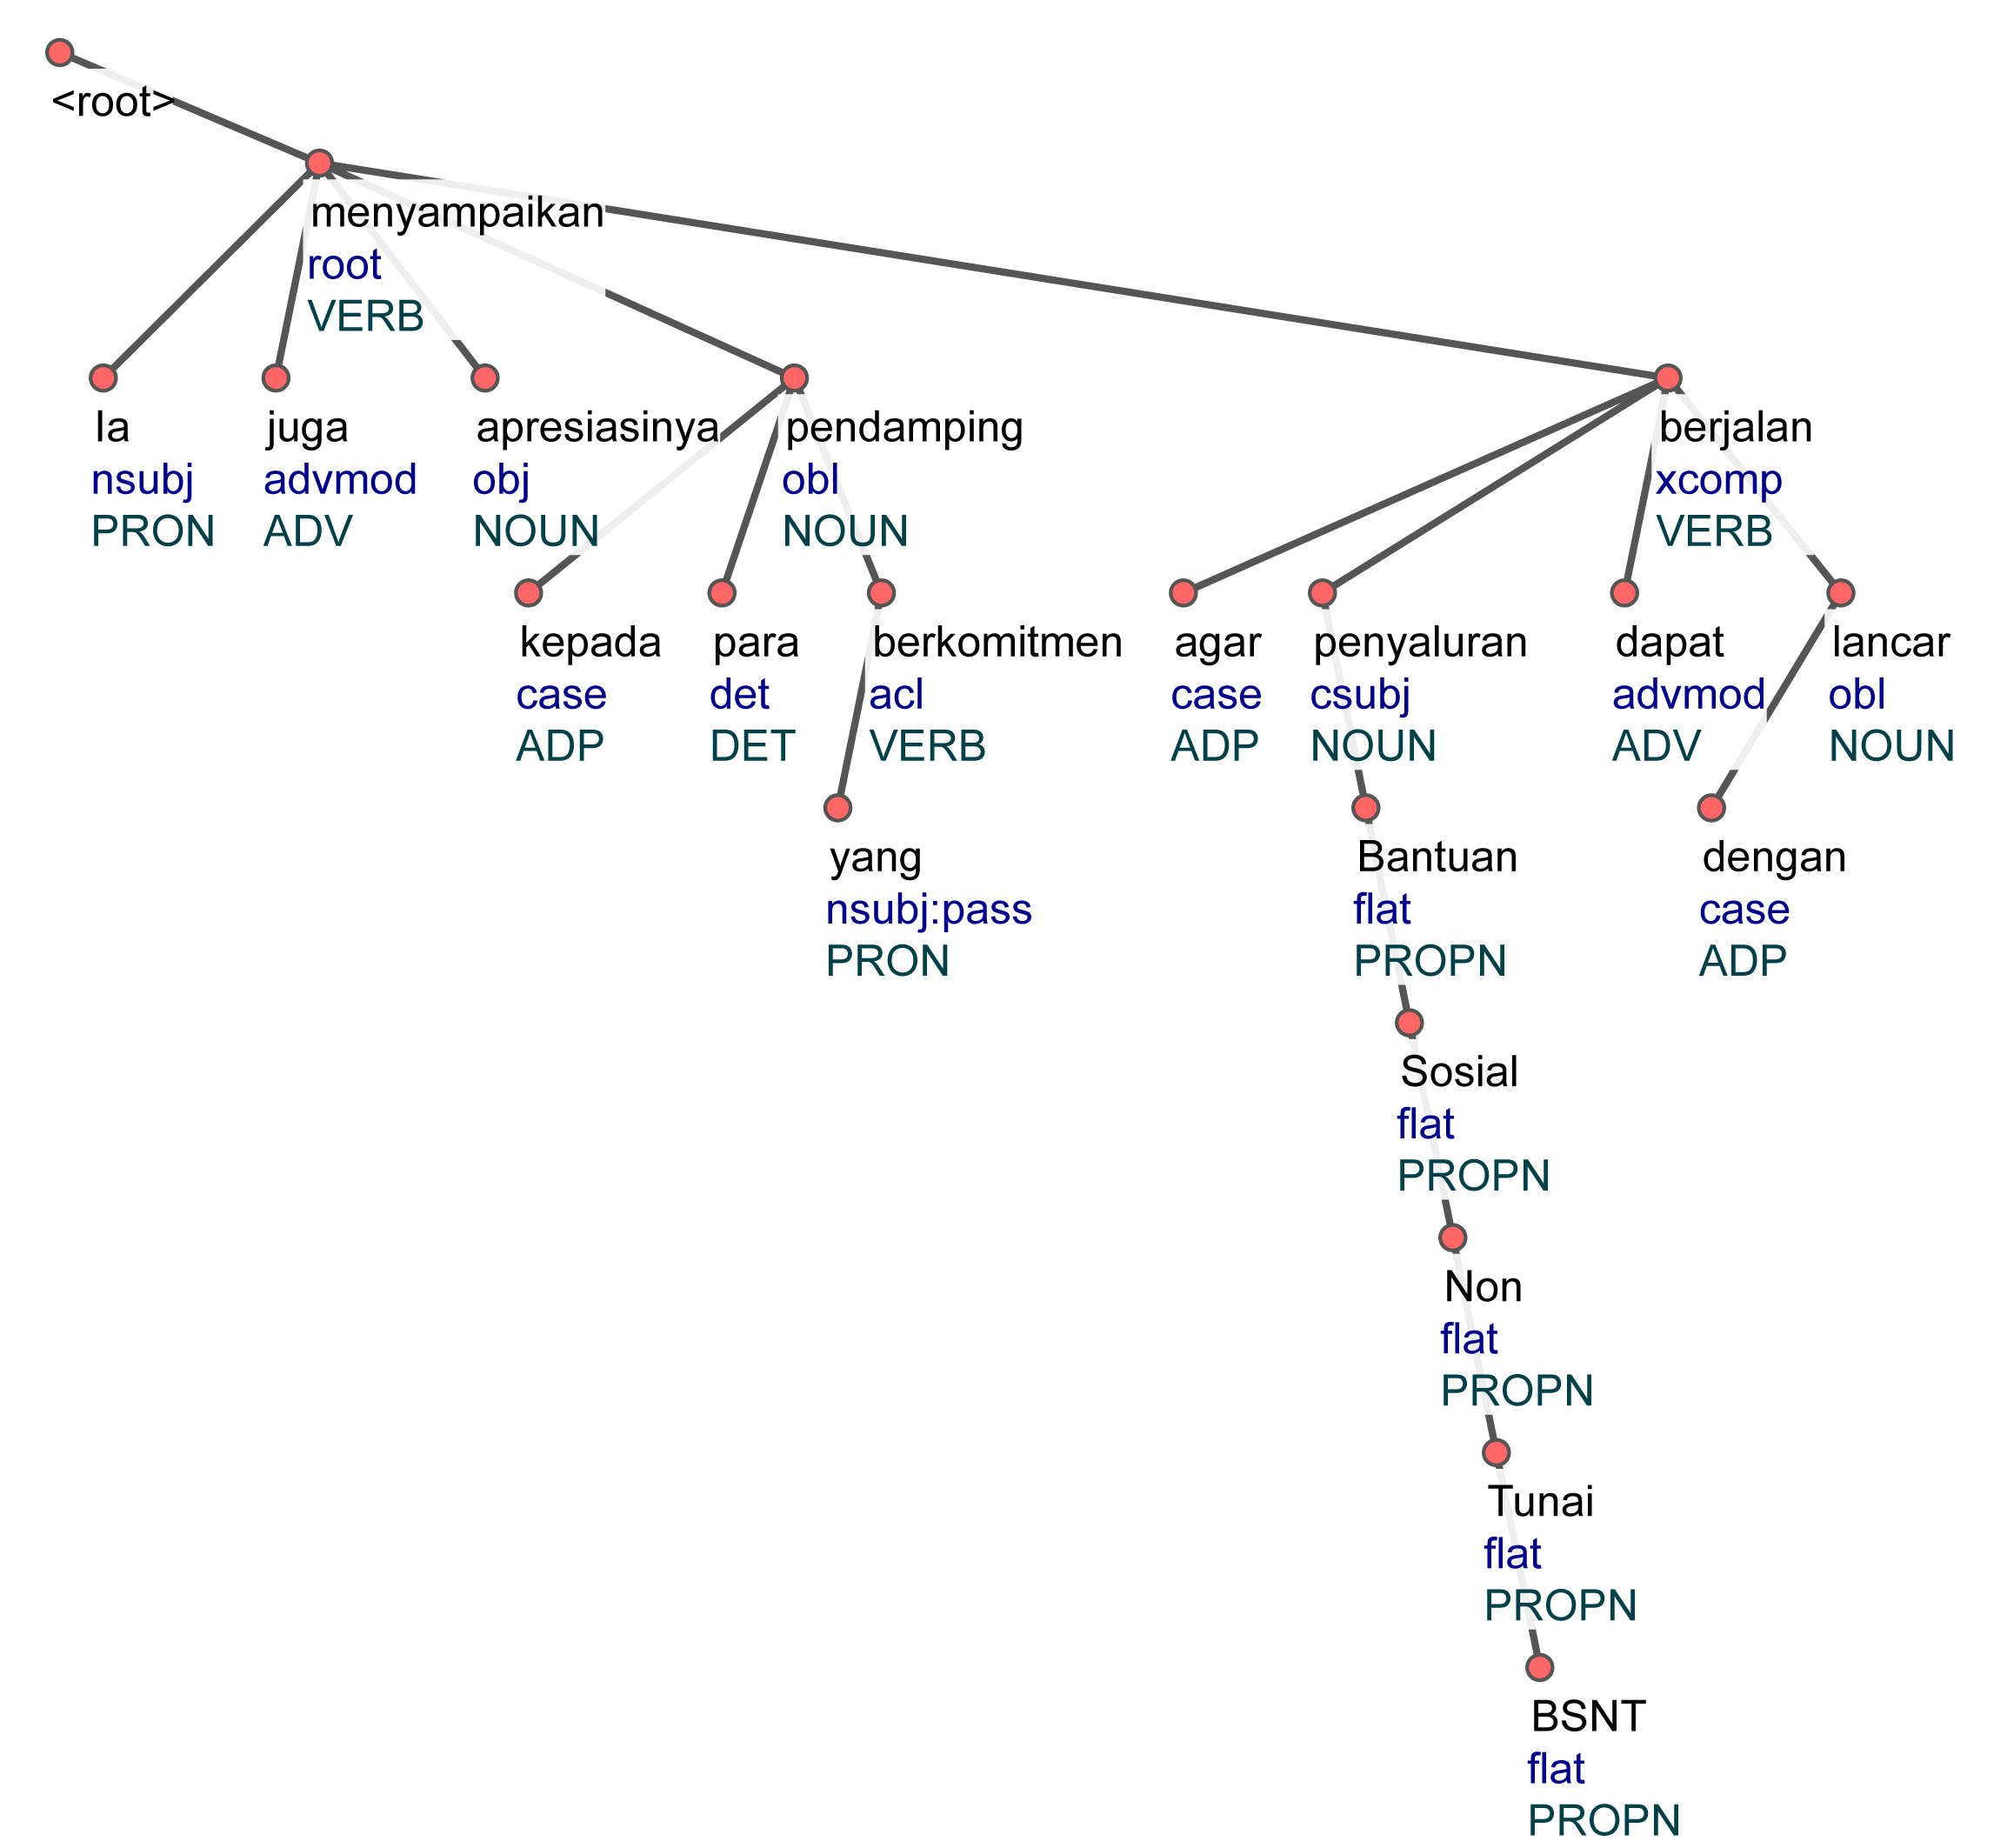
\includegraphics[width=0.8
	\textwidth] {pics/lampiran/lampirants3221.jpg} 
	\caption{Bank pohon struktur dependensi ragam tulis dokumen 3221} 
	\label{fig:lampirants3221} 
\end{figure}

%%

\begin{figure}
	\centering 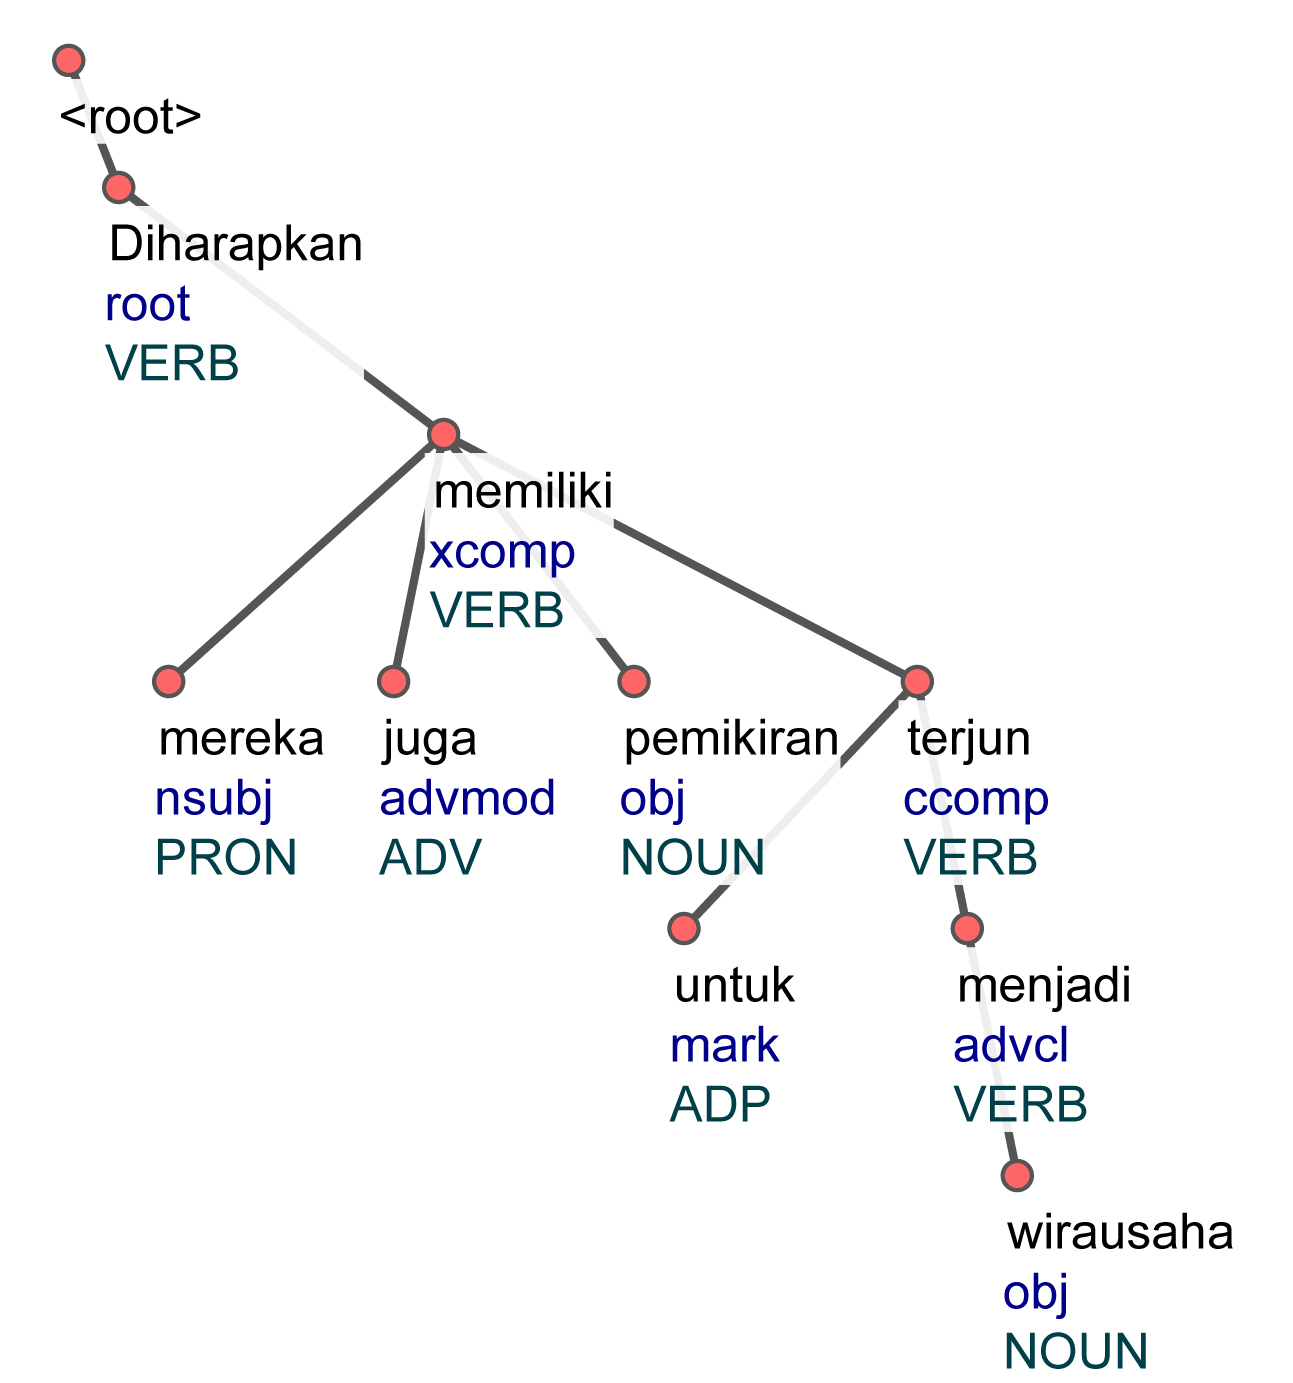
\includegraphics[width=0.45
	\textwidth] {pics/lampiran/lampirants4955.jpg} 
	\caption{Bank pohon struktur dependensi ragam tulis dokumen 4955} 
	\label{fig:lampirants4955} 
\end{figure}

\begin{figure}
	\centering 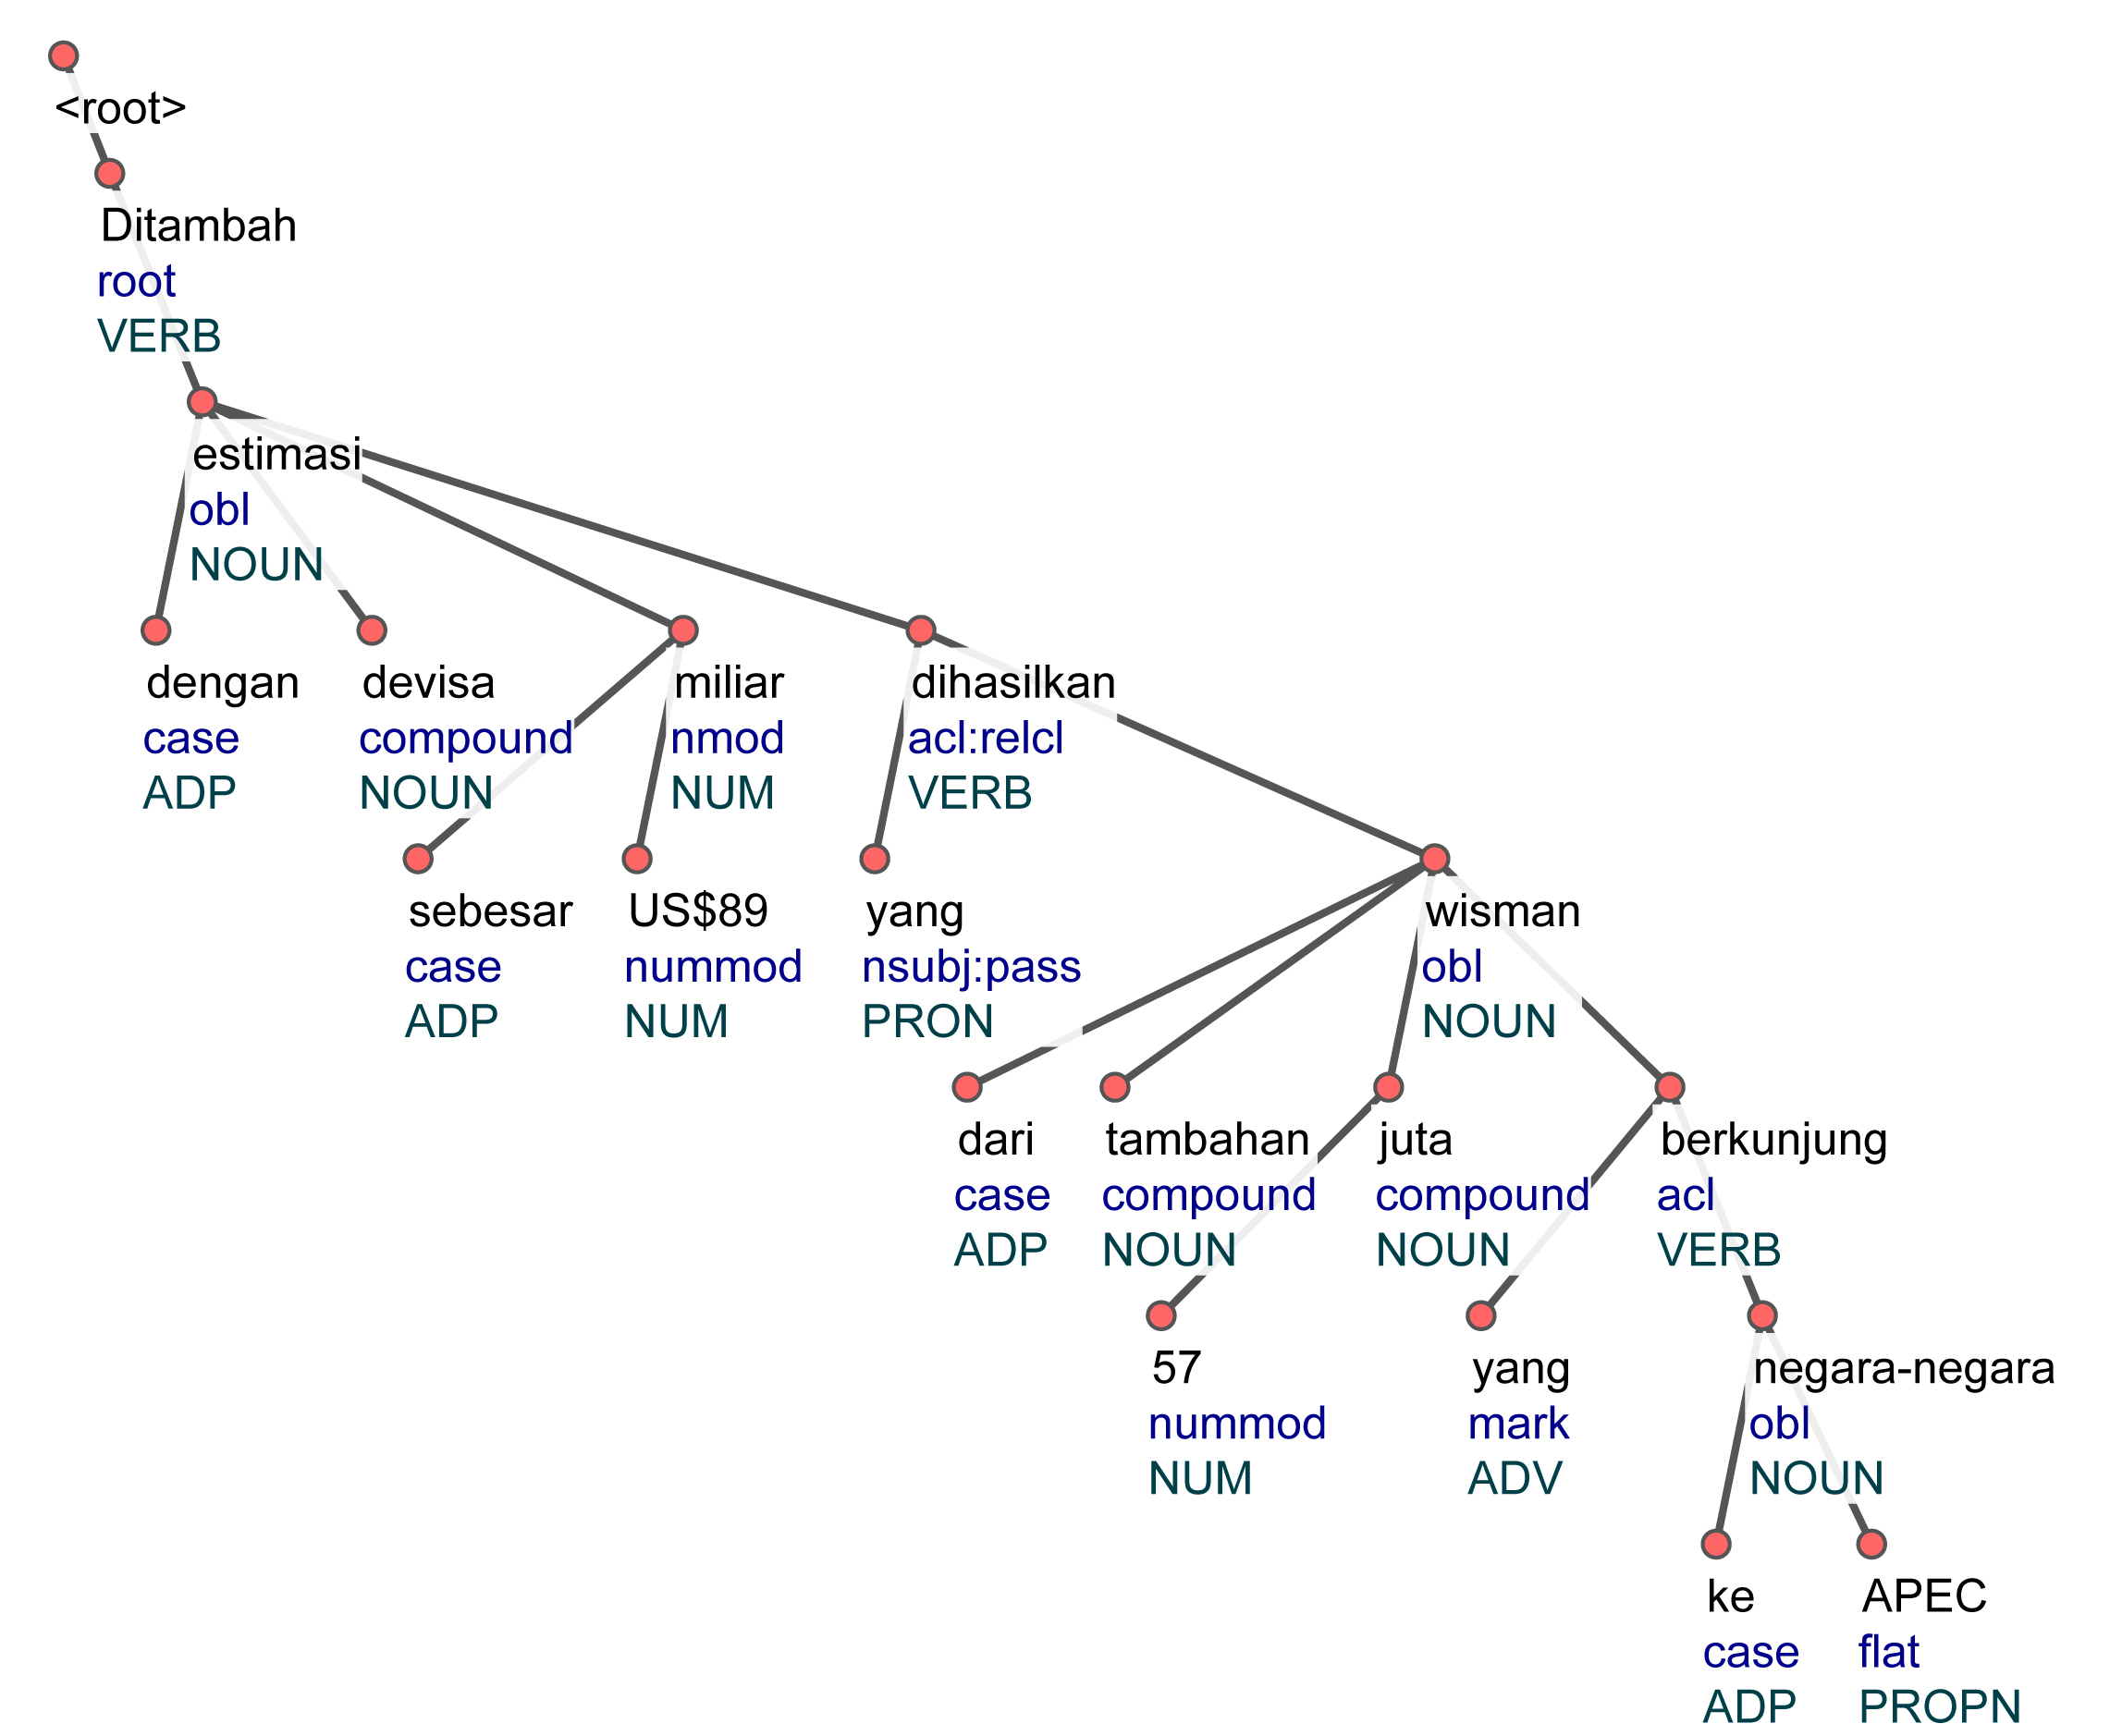
\includegraphics[width=0.8
	\textwidth] {pics/lampiran/lampirants5360.jpg} 
	\caption{Bank pohon struktur dependensi ragam tulis dokumen 5360} 
	\label{fig:lampirants5360} 
\end{figure}

\begin{figure}
	\centering 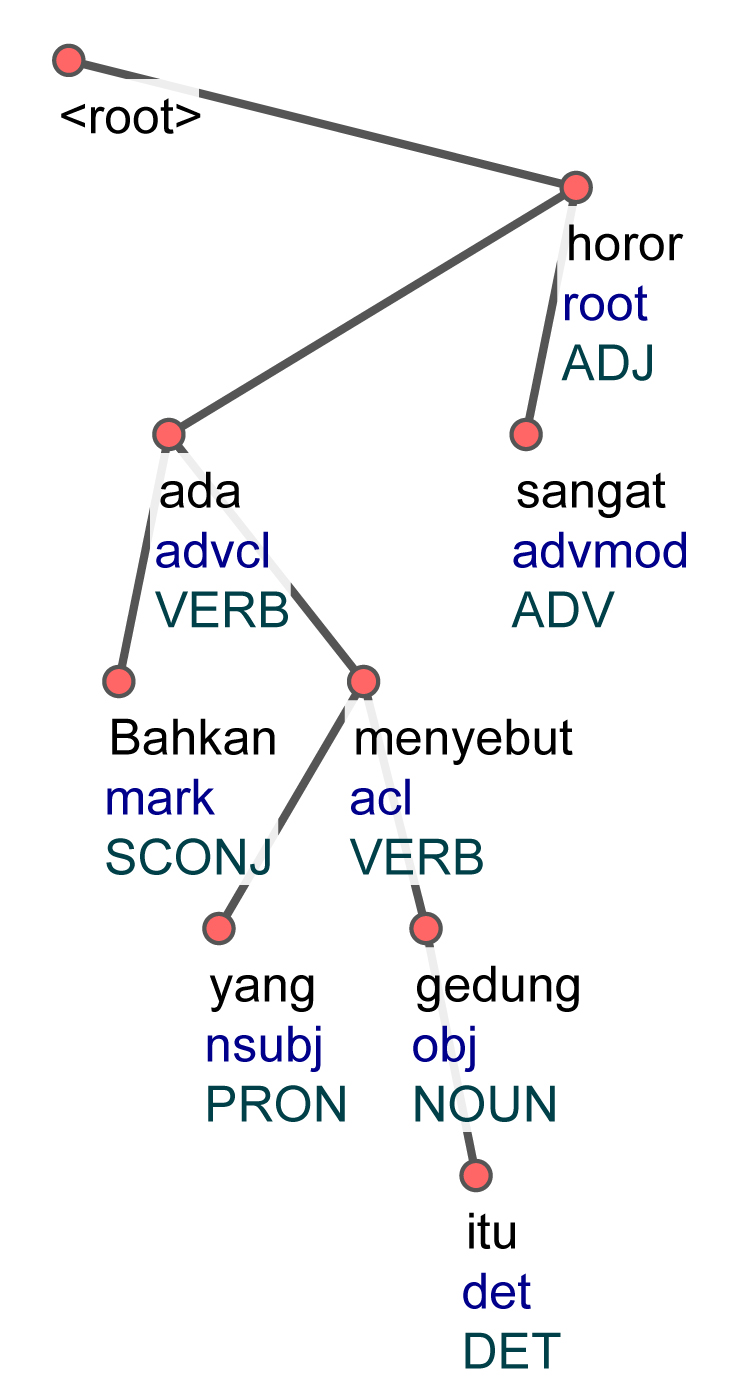
\includegraphics[width=0.25
	\textwidth] {pics/lampiran/lampirants5385.jpg} 
	\caption{Bank pohon struktur dependensi ragam tulis dokumen 5385} 
	\label{fig:lampirants5385} 
\end{figure}

\begin{figure}
	\centering 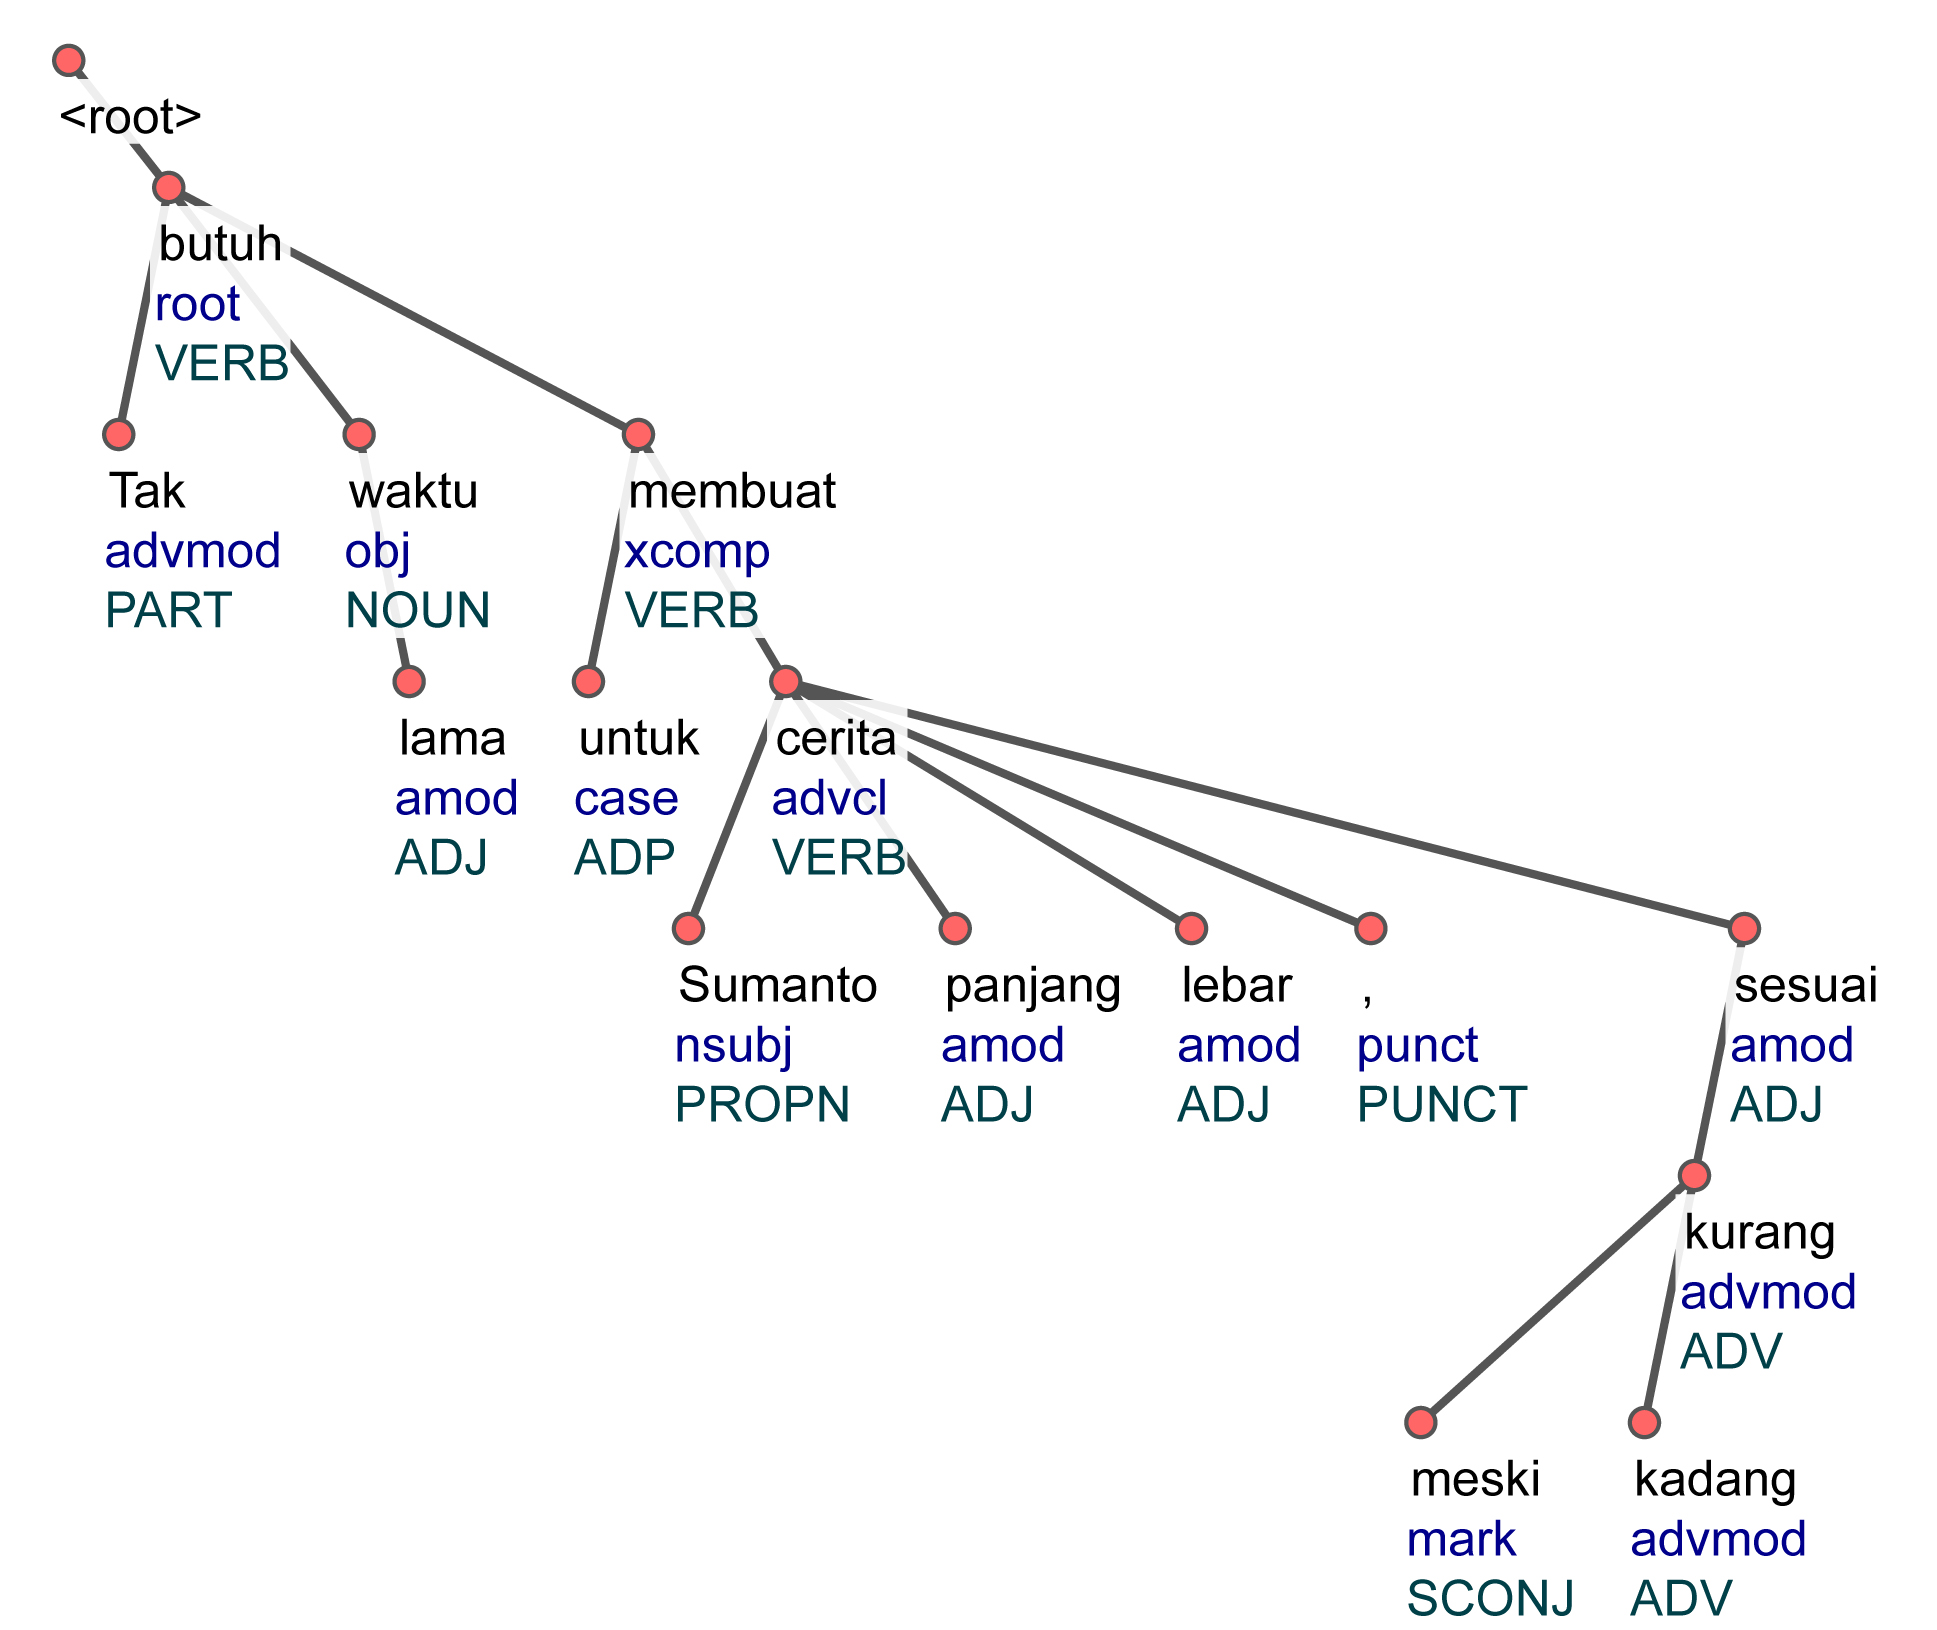
\includegraphics[width=0.7
	\textwidth] {pics/lampiran/lampirants6703.jpg} 
	\caption{Bank pohon struktur dependensi ragam tulis dokumen 6703} 
	\label{fig:lampirants6703} 
\end{figure}

\begin{figure}
	\centering 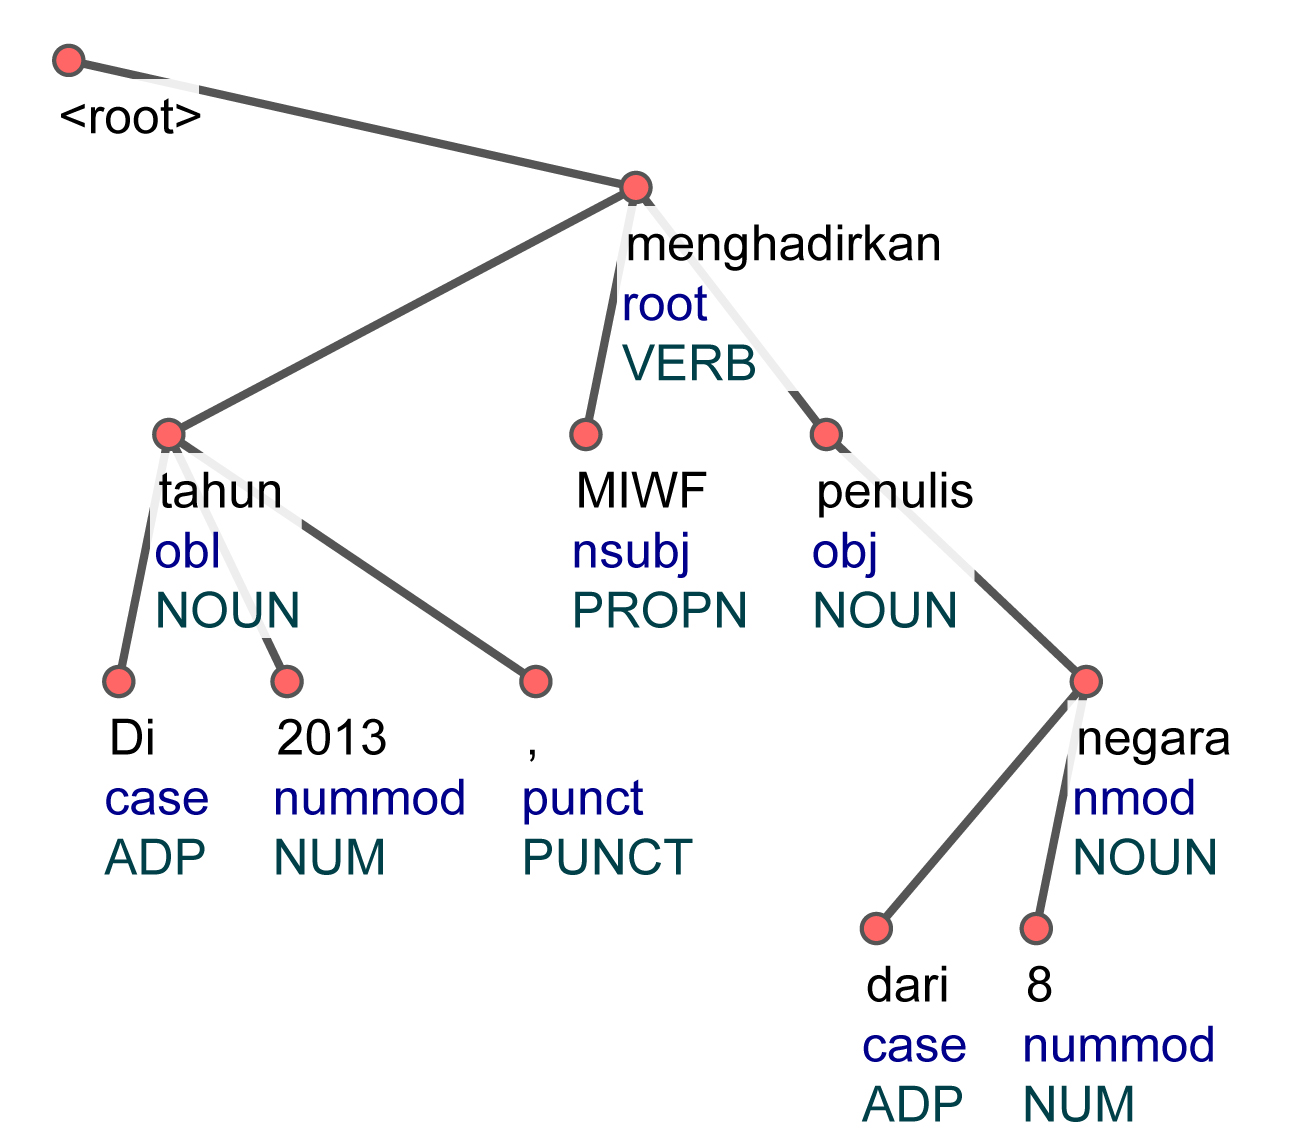
\includegraphics[width=0.45
	\textwidth] {pics/lampiran/lampirants7706.jpg} 
	\caption{Bank pohon struktur dependensi ragam tulis dokumen 7706} 
	\label{fig:lampirants7706} 
\end{figure}

%%

\begin{figure}
	\centering 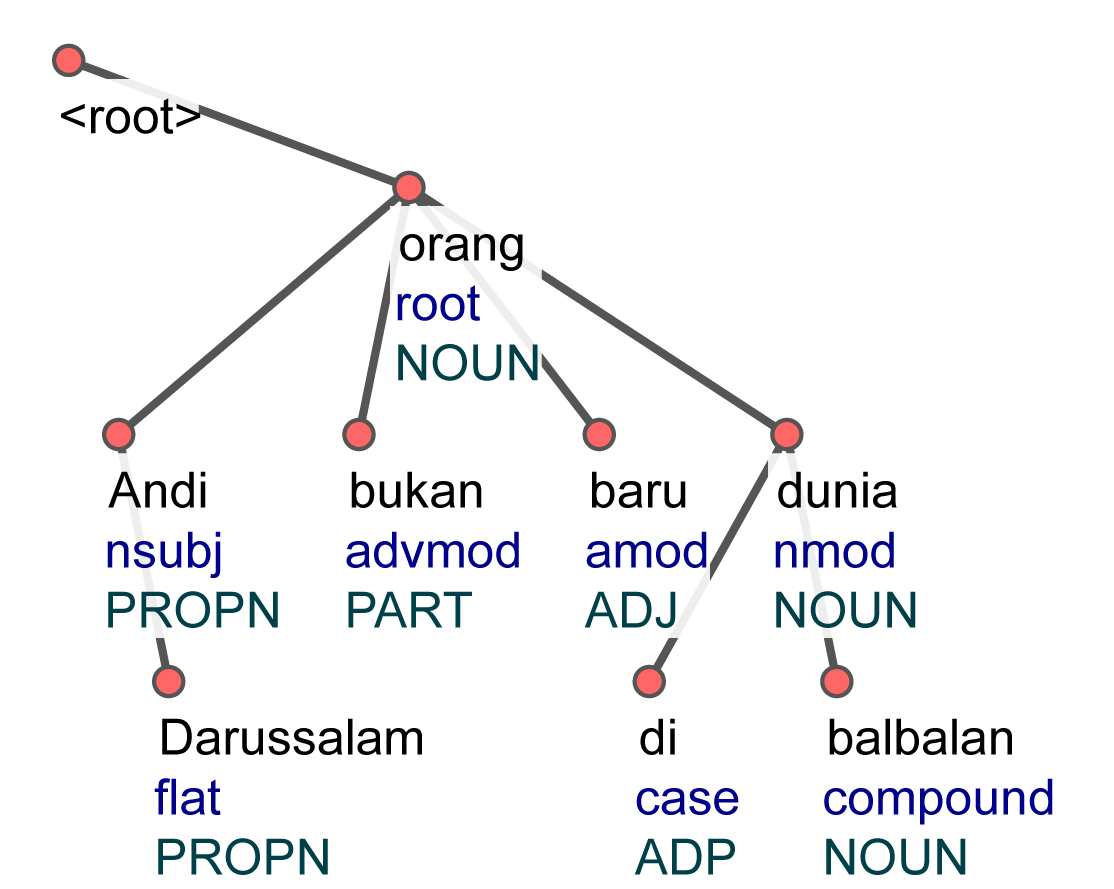
\includegraphics[width=0.4
	\textwidth] {pics/lampiran/lampirants8990.jpg} 
	\caption{Bank pohon struktur dependensi ragam tulis dokumen 8990} 
	\label{fig:lampirants8990} 
\end{figure}

\begin{figure}
	\centering 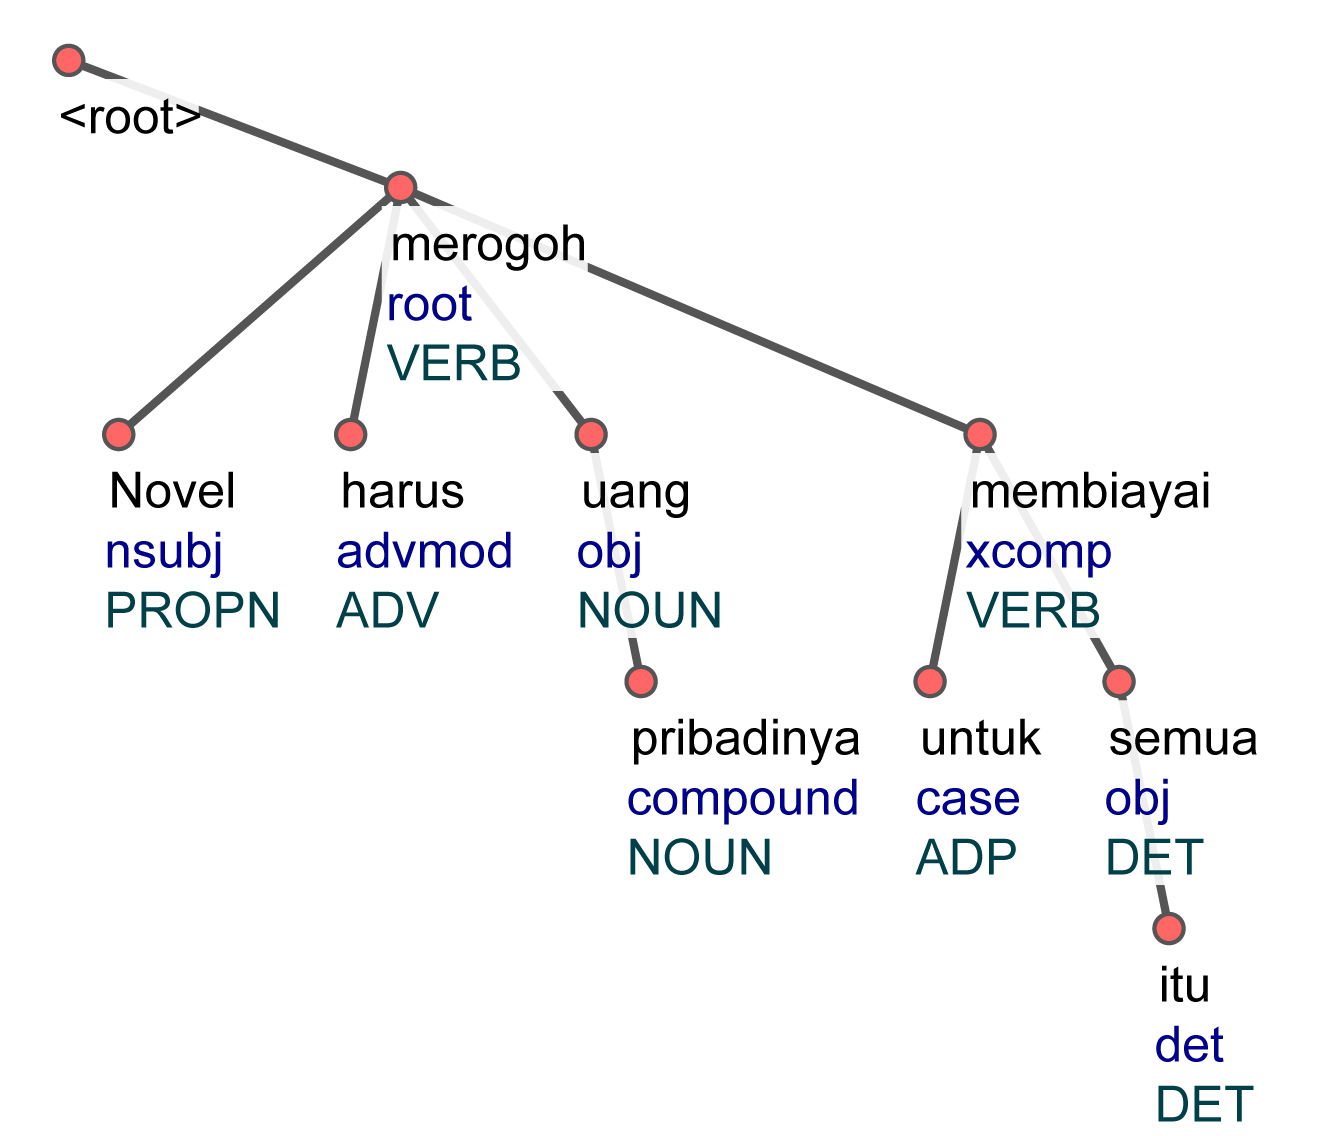
\includegraphics[width=0.5
	\textwidth] {pics/lampiran/lampirants9184.jpg} 
	\caption{Bank pohon struktur dependensi ragam tulis dokumen 9184} 
	\label{fig:lampirants9184} 
\end{figure}


%-----------------------------------------------------------------------------%
\addChapter{Contoh bank pohon struktur dependensi ragam lisan}
\chapter*{Lampiran 2: Contoh Bank Pohon Struktur Dependensi Ragam Lisan}
%-----------------------------------------------------------------------------%

\begin{figure}
	\centering 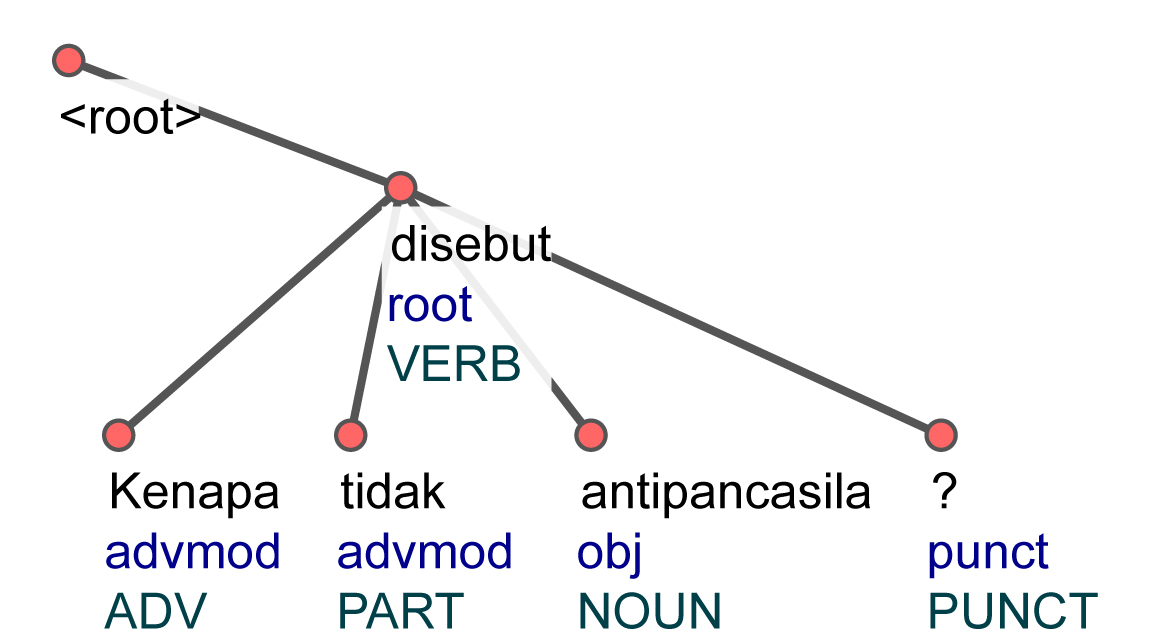
\includegraphics[width=0.4
	\textwidth] {pics/lampiran/lampiranls100.jpg} 
	\caption{Bank pohon struktur dependensi ragam lisan dokumen 100} 
	\label{fig:lampiranls100} 
\end{figure}

\begin{figure}
	\centering 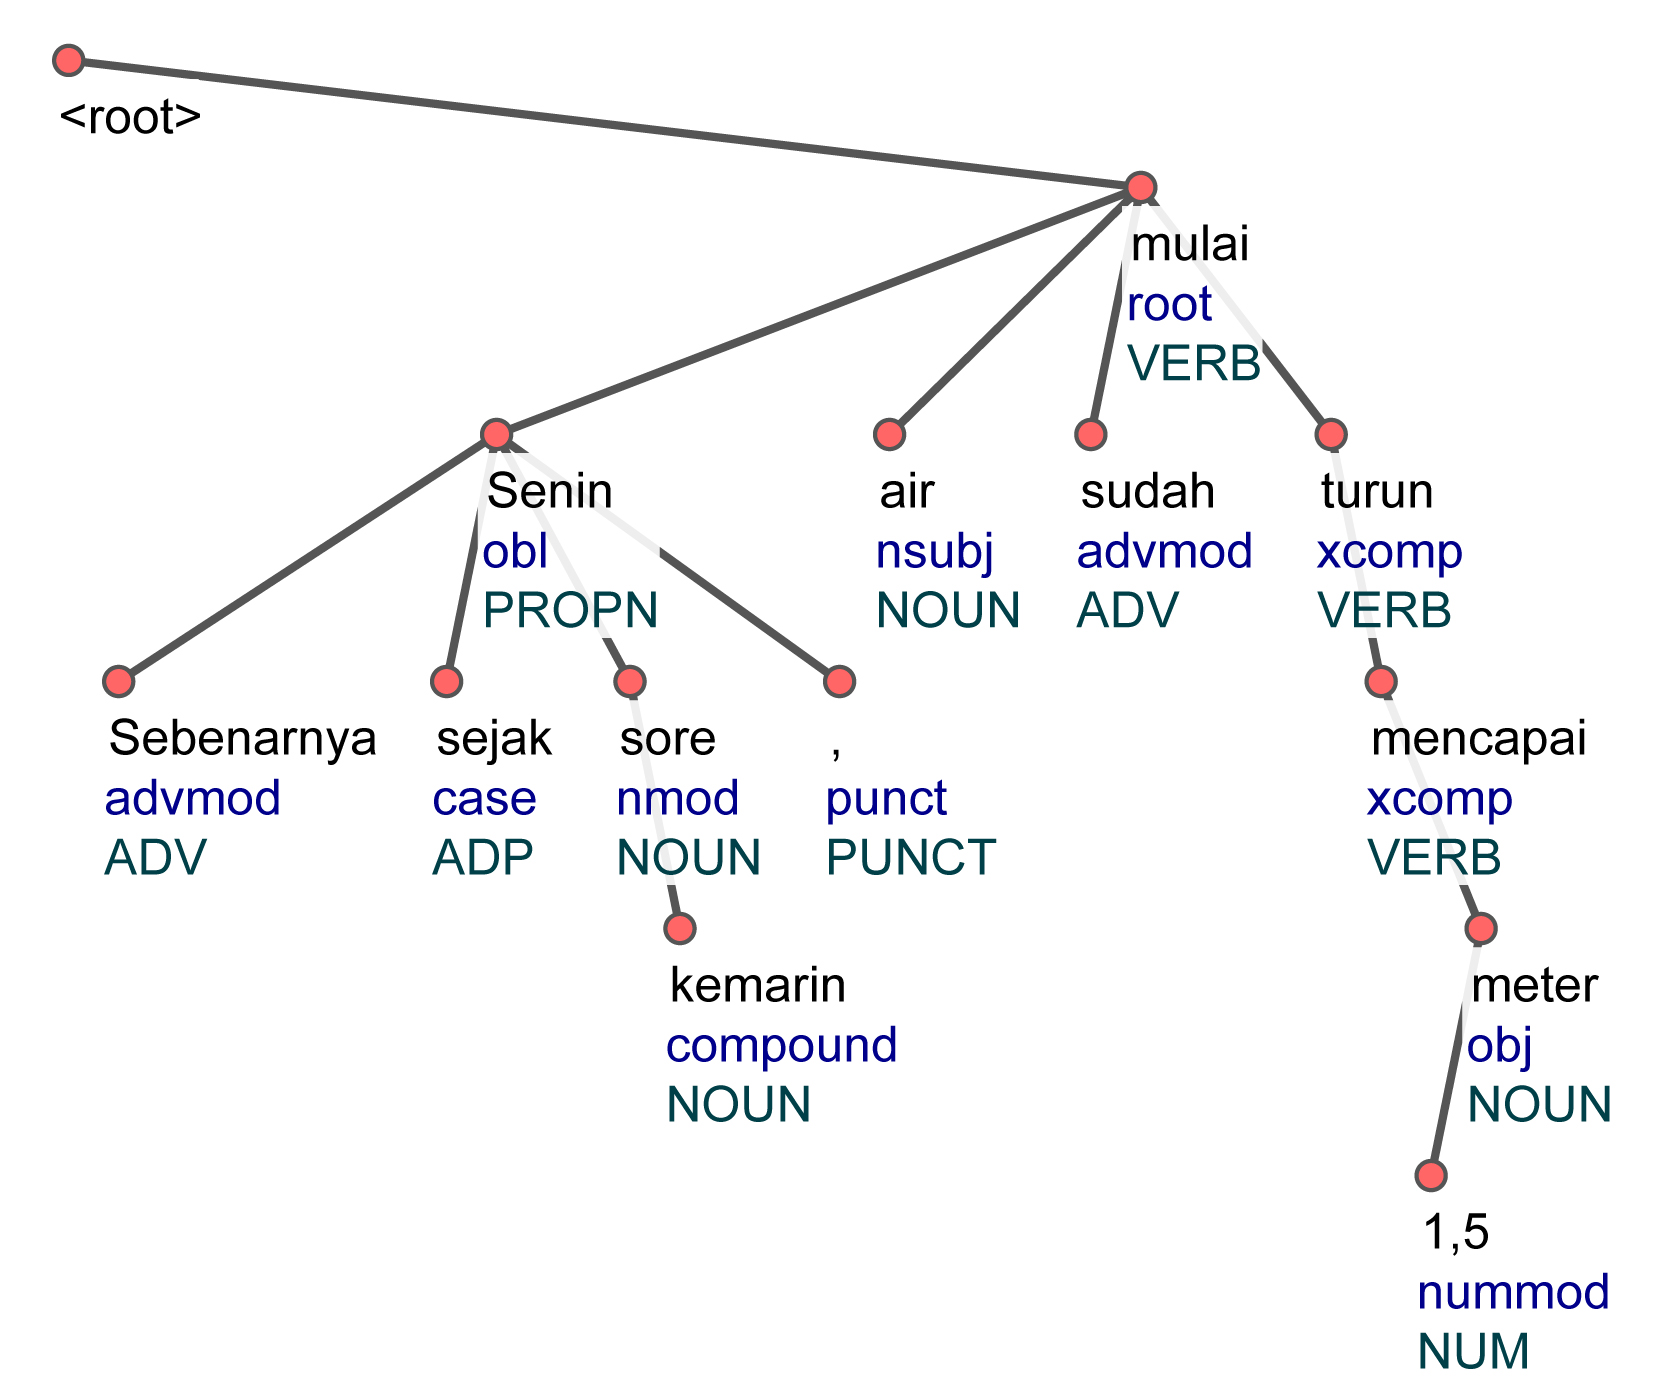
\includegraphics[width=0.6
	\textwidth] {pics/lampiran/lampiranls592.jpg} 
	\caption{Bank pohon struktur dependensi ragam lisan dokumen 592} 
	\label{fig:lampiranls592} 
\end{figure}

\begin{figure}
	\centering 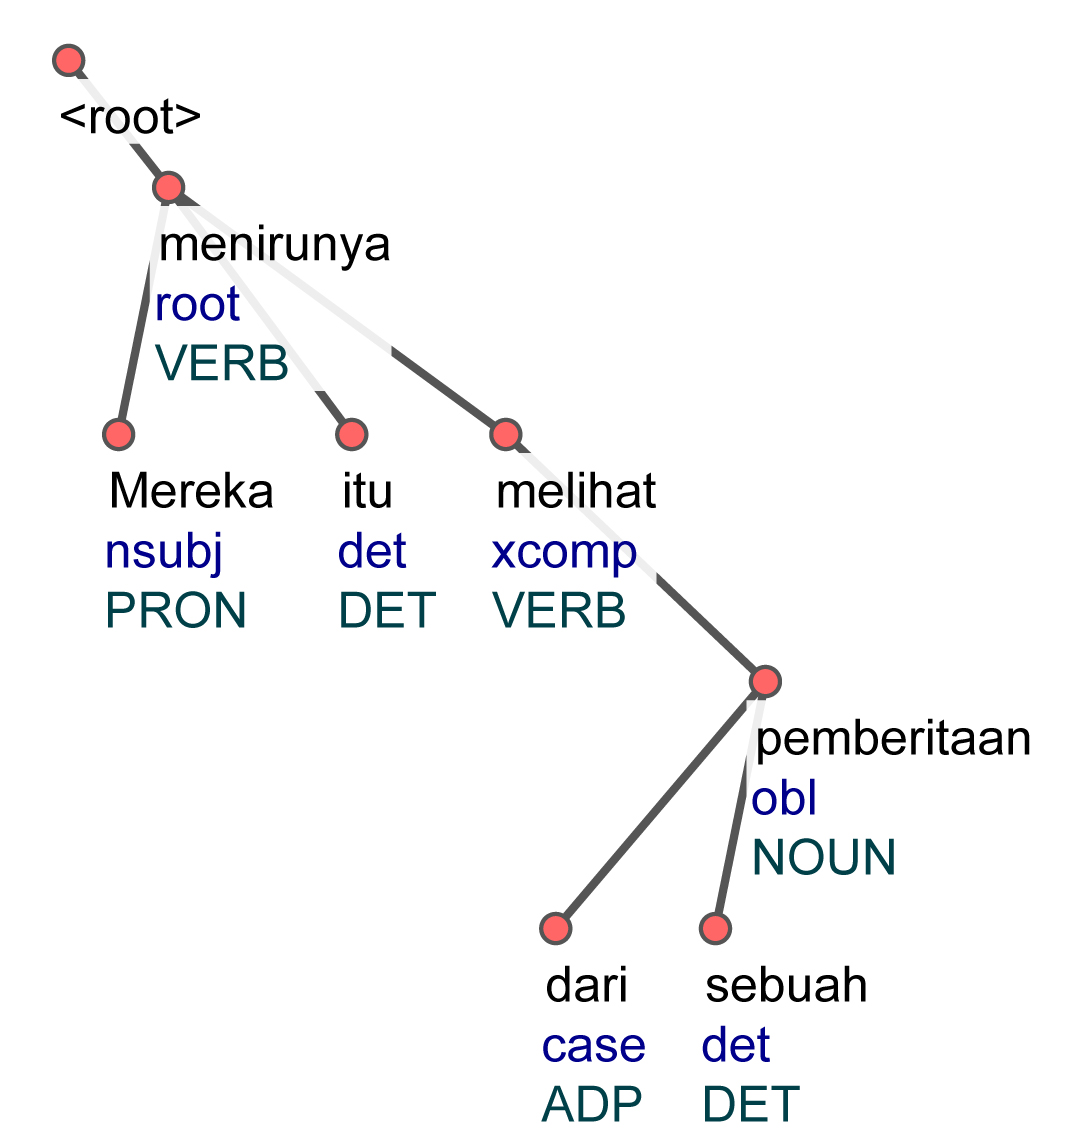
\includegraphics[width=0.4
	\textwidth] {pics/lampiran/lampiranls1100.jpg} 
	\caption{Bank pohon struktur dependensi ragam lisan dokumen 1100} 
	\label{fig:lampiranls1100} 
\end{figure}

\begin{figure}
	\centering 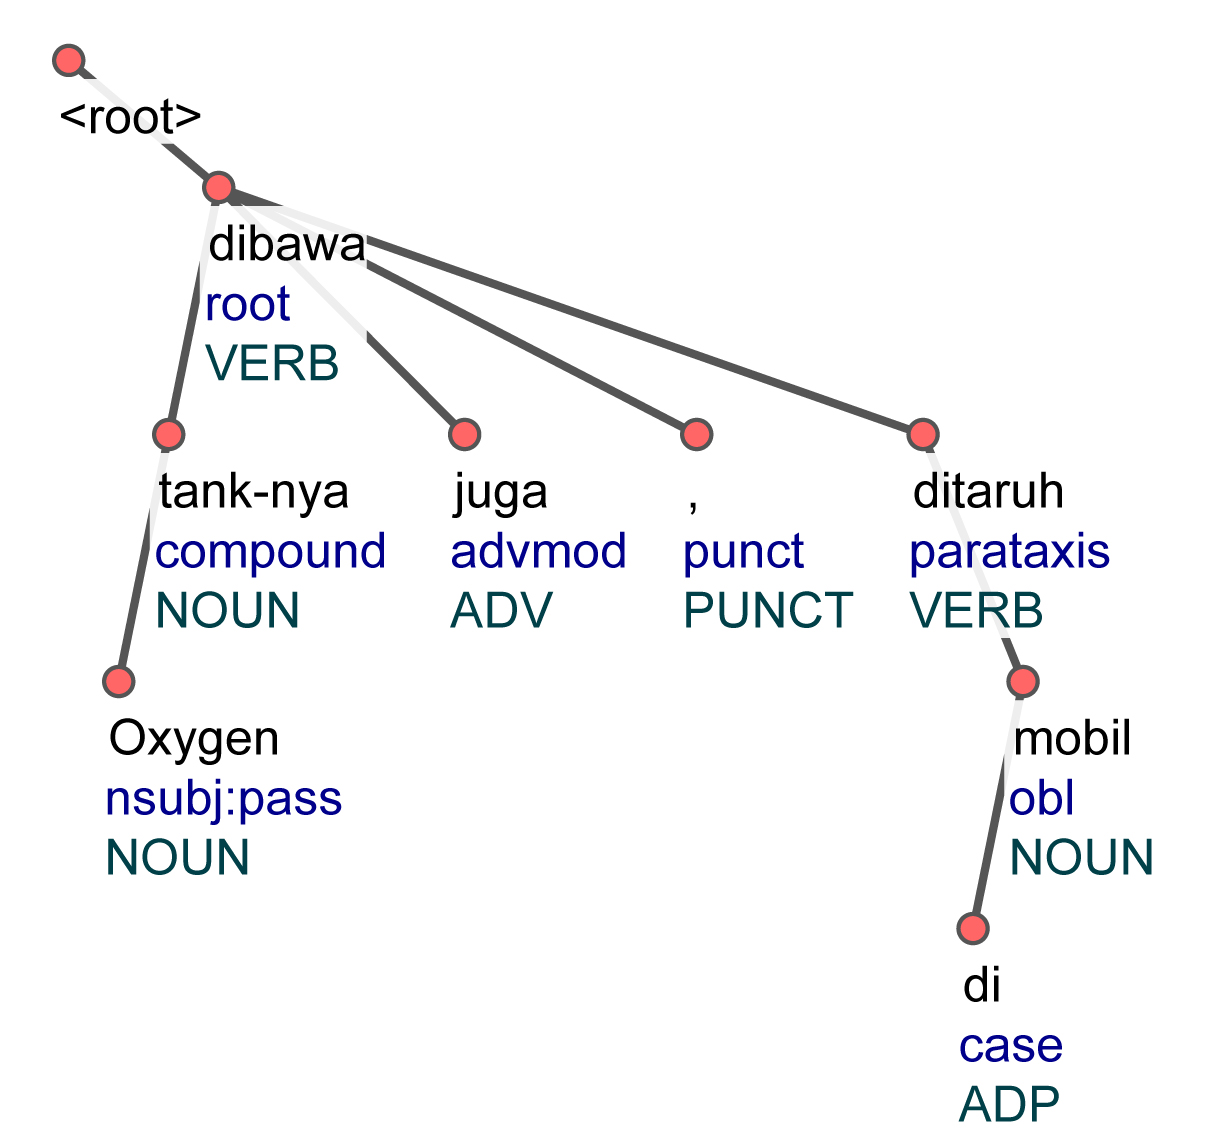
\includegraphics[width=0.45
	\textwidth] {pics/lampiran/lampiranls1836.jpg} 
	\caption{Bank pohon struktur dependensi ragam lisan dokumen 1836} 
	\label{fig:lampiranls1836} 
\end{figure}

\begin{figure}
	\centering 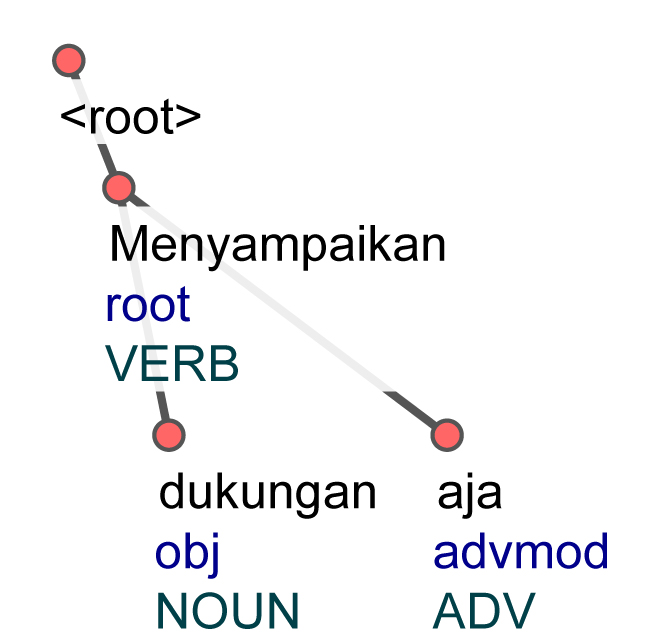
\includegraphics[width=0.3
	\textwidth] {pics/lampiran/lampiranls1928.jpg} 
	\caption{Bank pohon struktur dependensi ragam lisan dokumen 1928} 
	\label{fig:lampiranls1928} 
\end{figure}

%%

\begin{figure}
	\centering 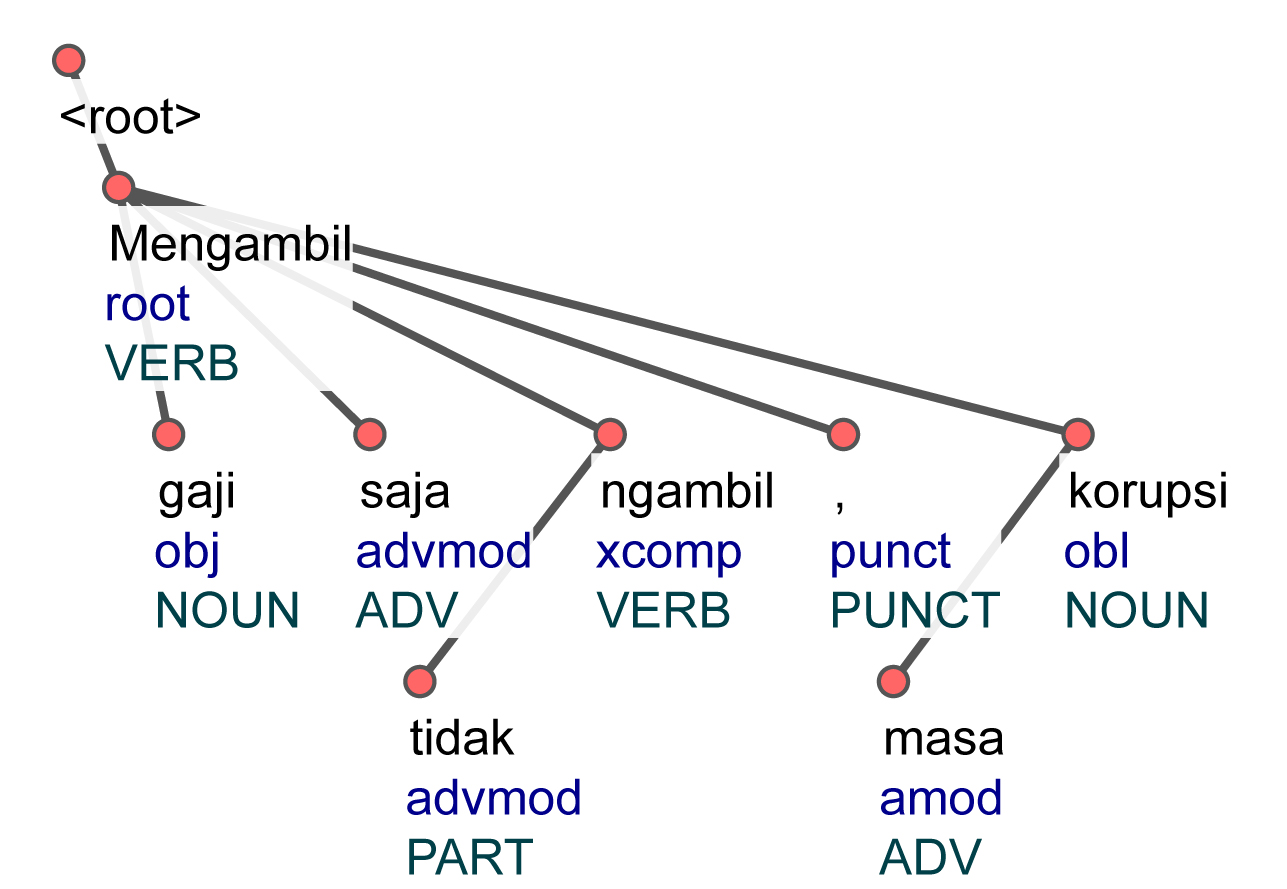
\includegraphics[width=0.45
	\textwidth] {pics/lampiran/lampiranls3530.jpg} 
	\caption{Bank pohon struktur dependensi ragam lisan dokumen 3530} 
	\label{fig:lampiranls3530} 
\end{figure}

\begin{figure}
	\centering 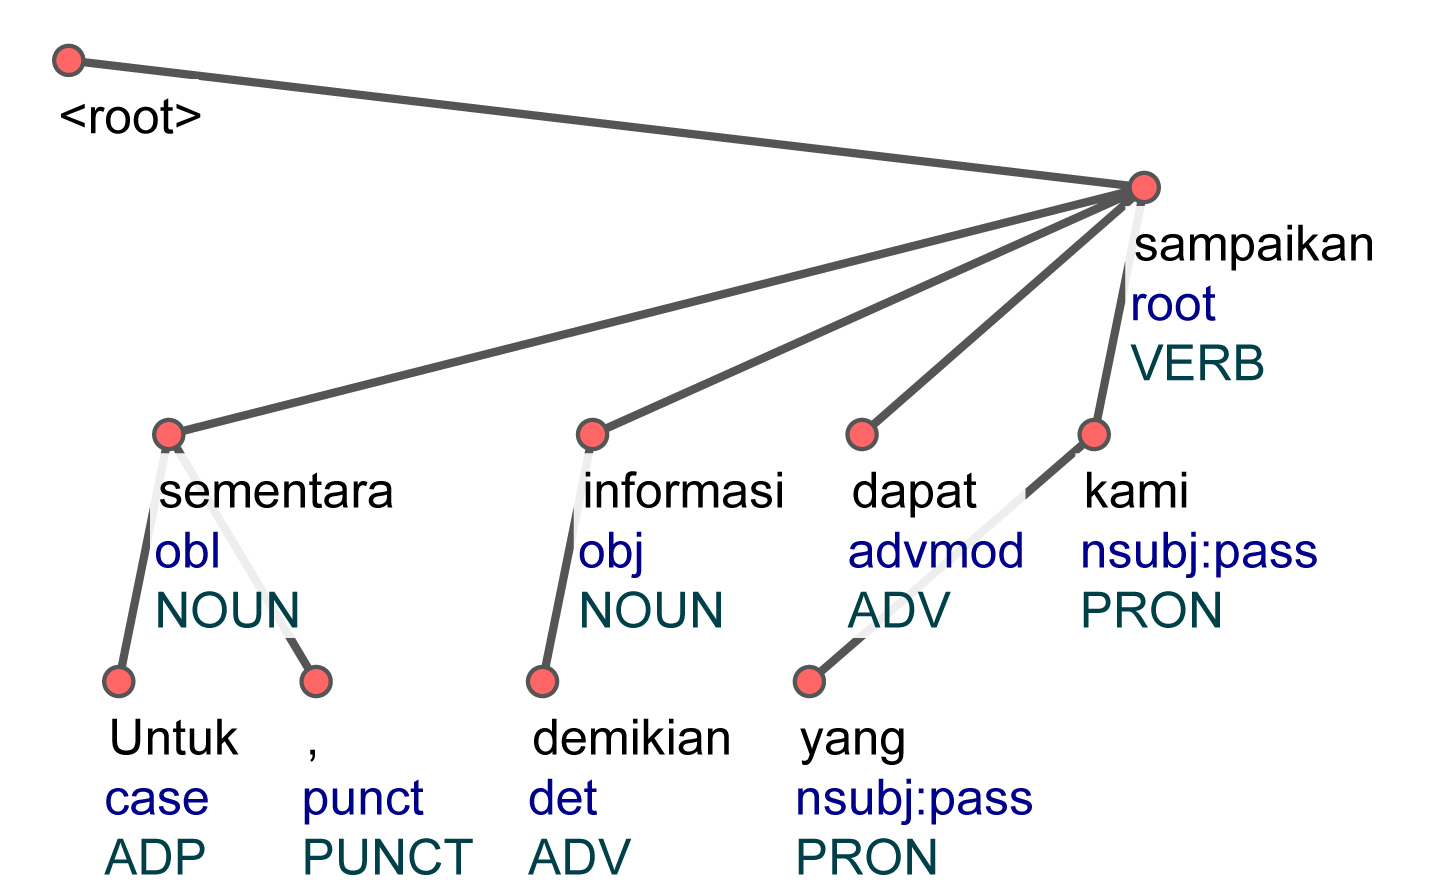
\includegraphics[width=0.5
	\textwidth] {pics/lampiran/lampiranls4327.jpg} 
	\caption{Bank pohon struktur dependensi ragam lisan dokumen 4327} 
	\label{fig:lampiranls4327} 
\end{figure}

\begin{figure}
	\centering 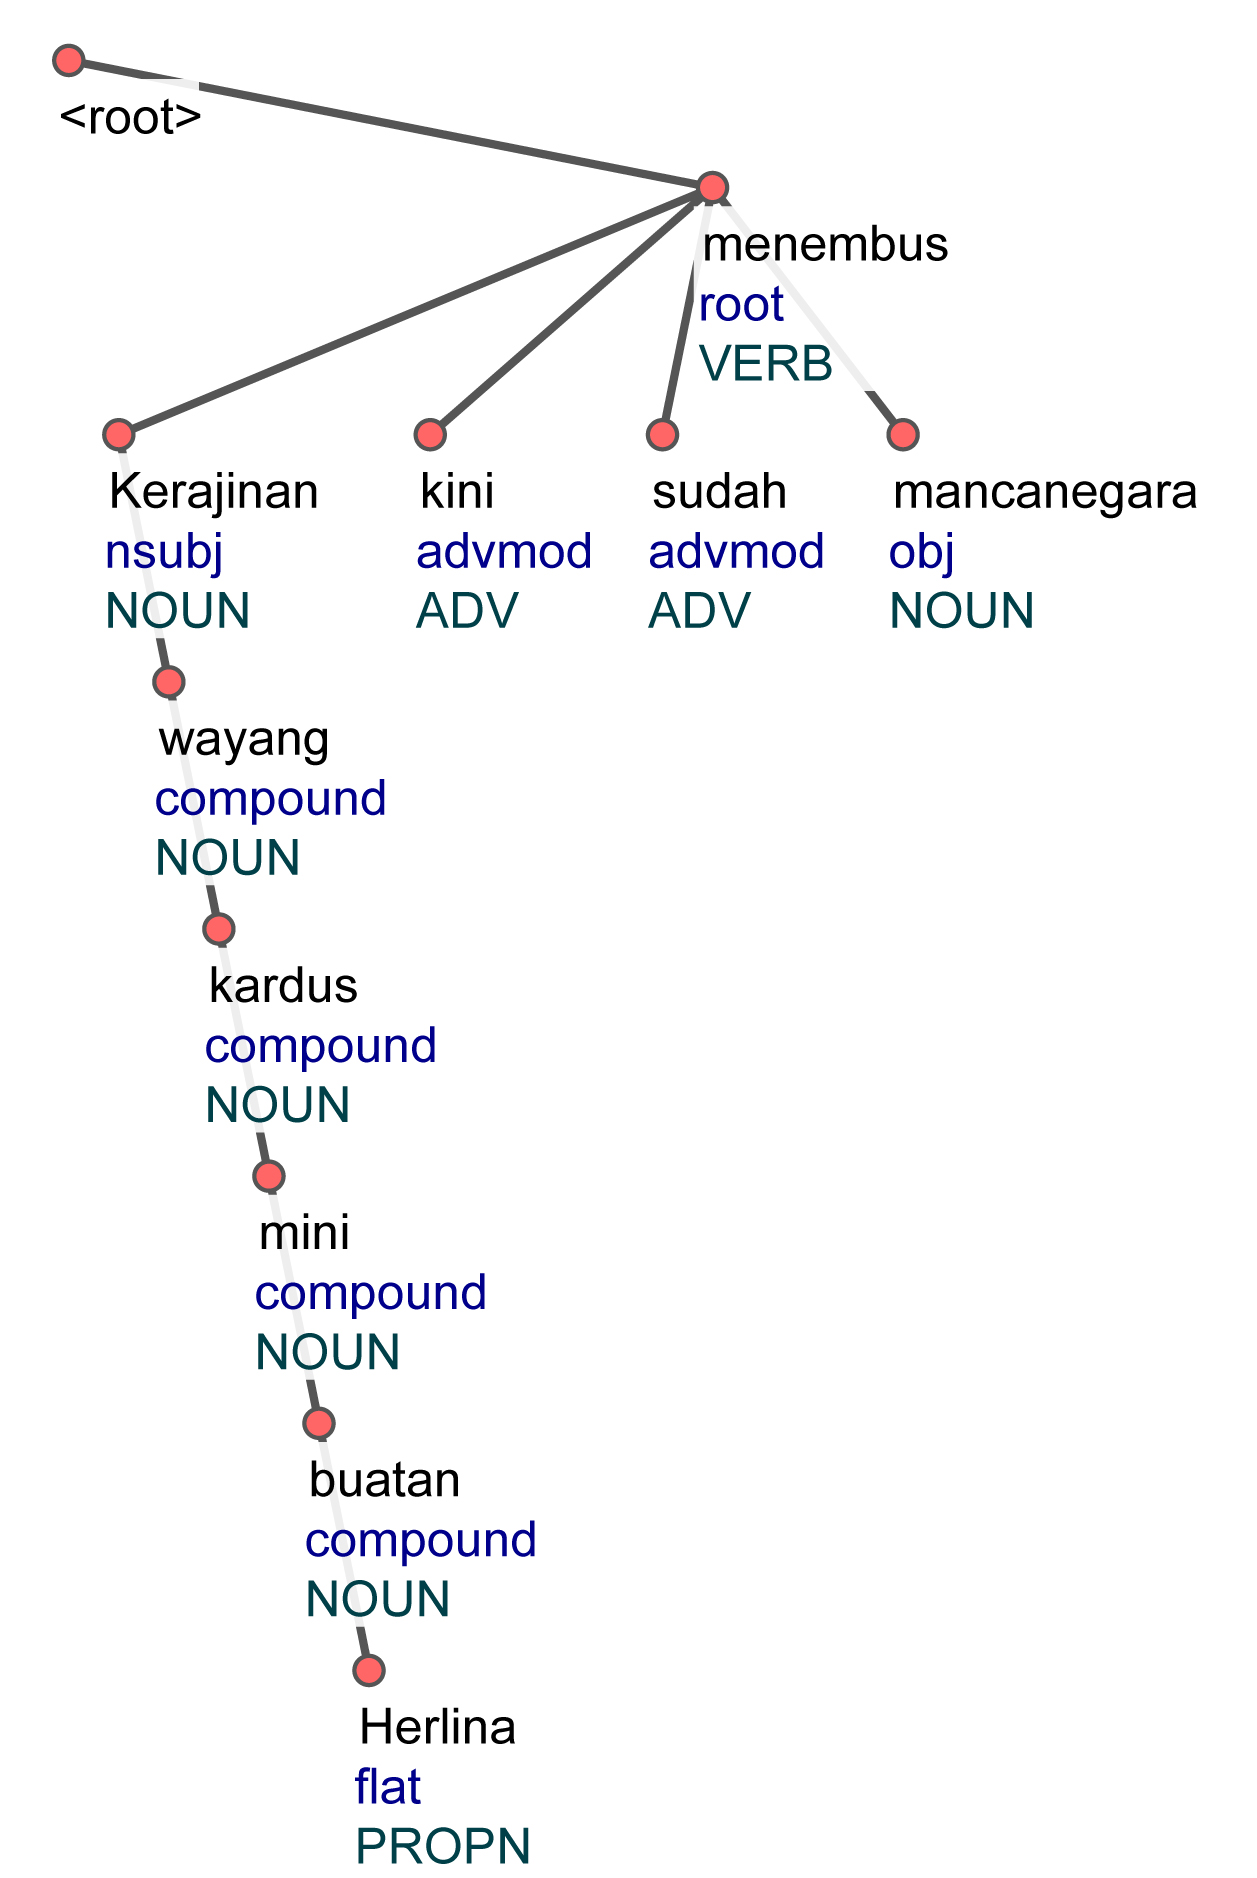
\includegraphics[width=0.45
	\textwidth] {pics/lampiran/lampiranls4991.jpg} 
	\caption{Bank pohon struktur dependensi ragam lisan dokumen 4991} 
	\label{fig:lampiranls4991} 
\end{figure}

\begin{figure}
	\centering 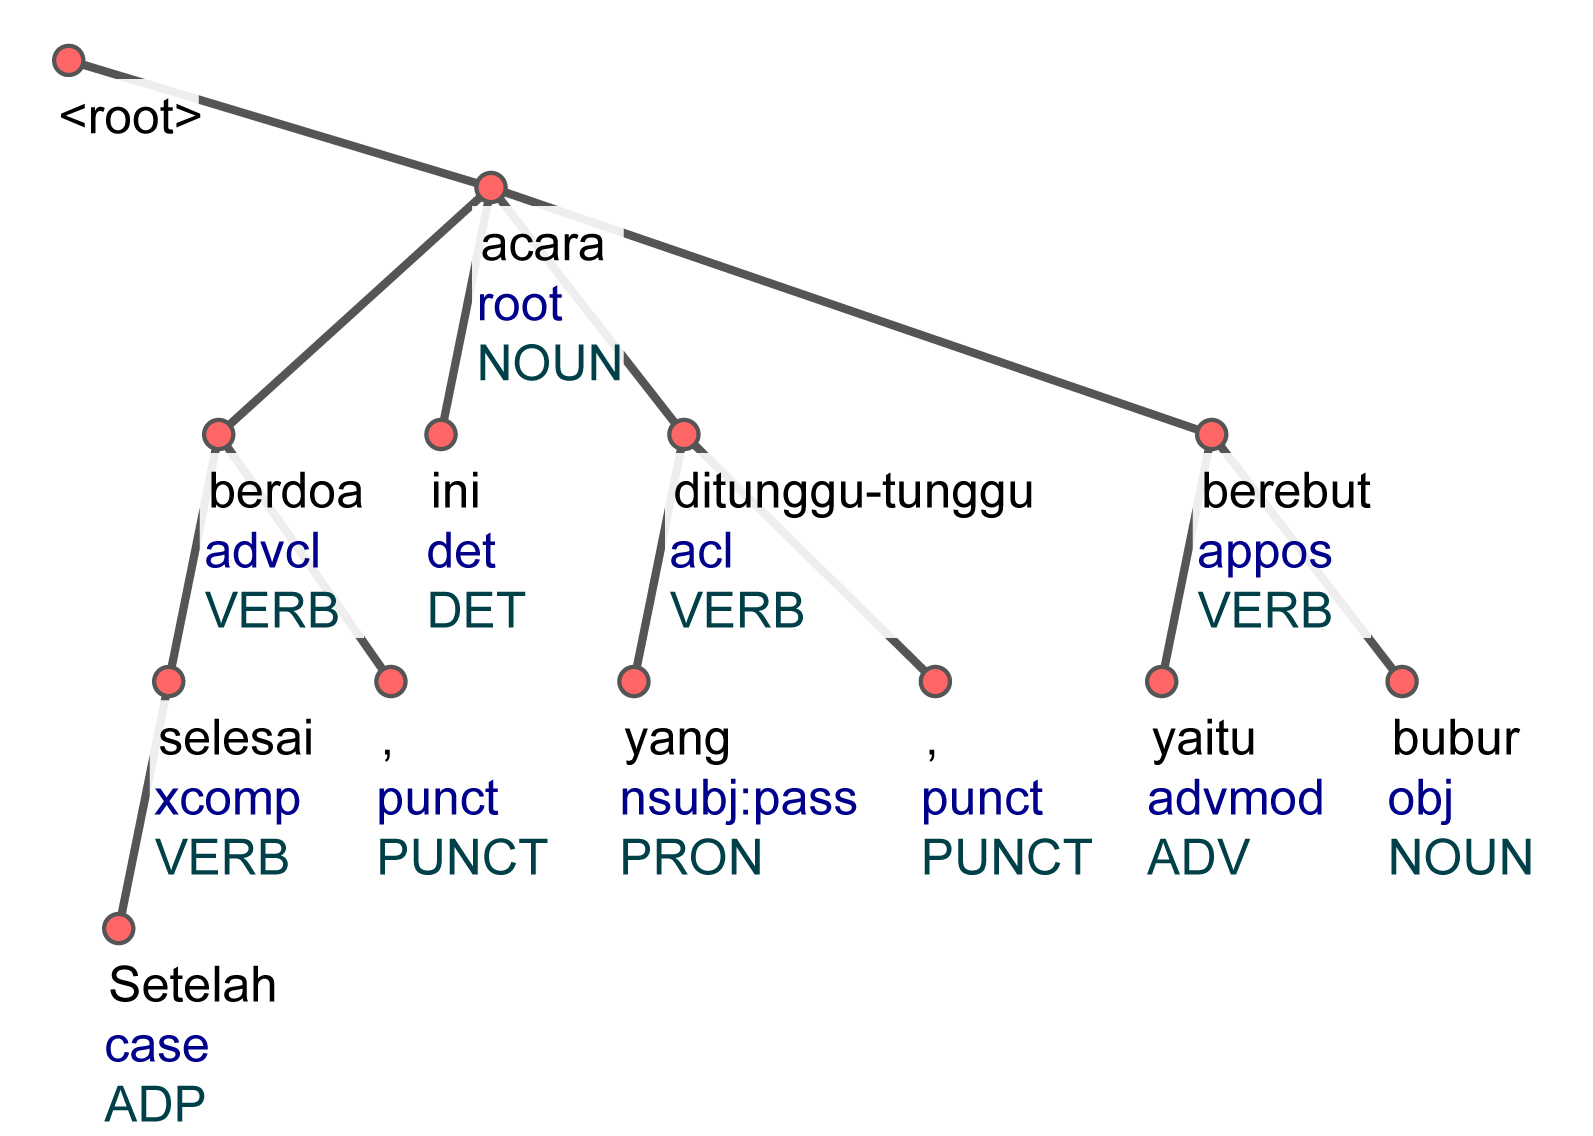
\includegraphics[width=0.6
	\textwidth] {pics/lampiran/lampiranls5677.jpg} 
	\caption{Bank pohon struktur dependensi ragam lisan dokumen 5677} 
	\label{fig:lampiranls5677} 
\end{figure}

\begin{figure}
	\centering 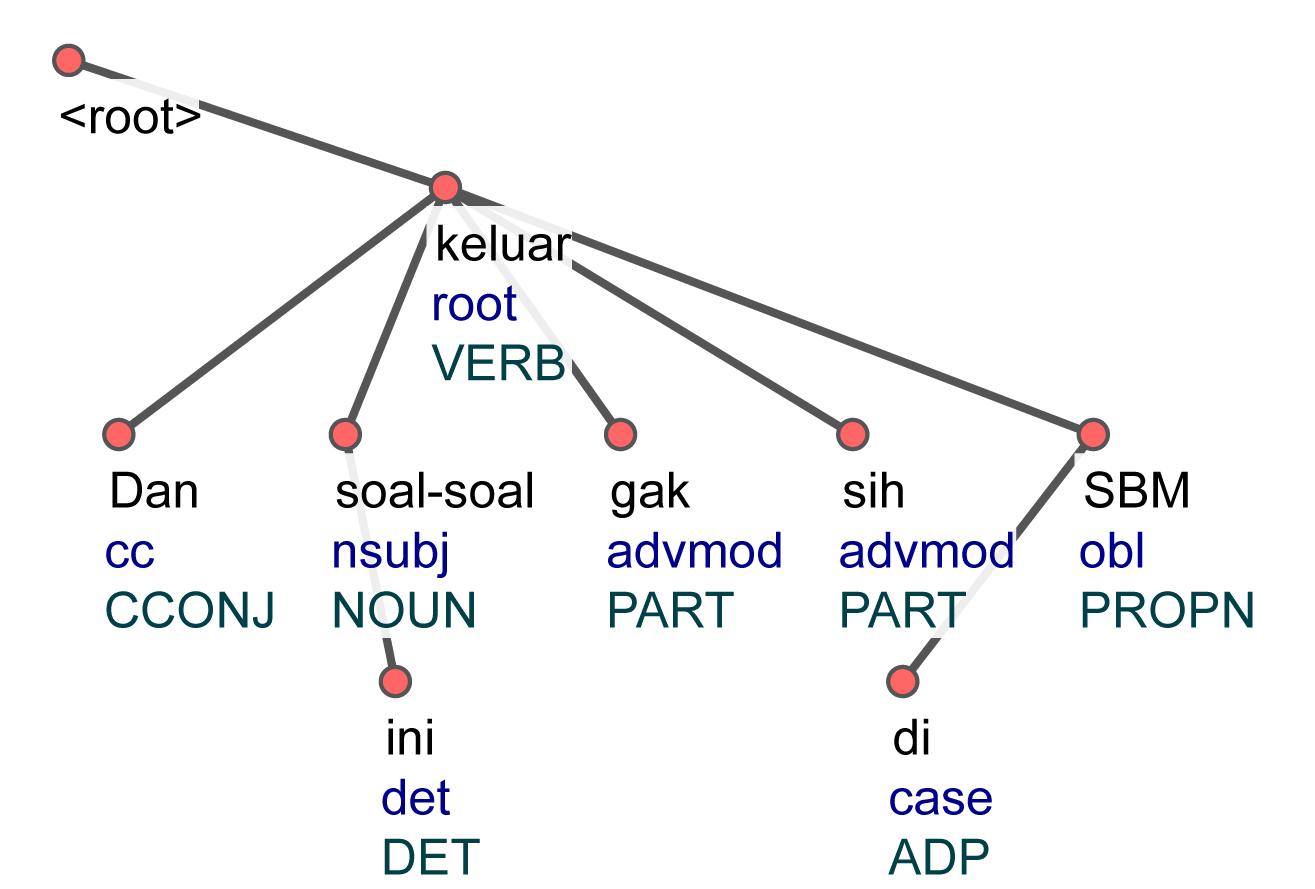
\includegraphics[width=0.5
	\textwidth] {pics/lampiran/lampiranls7047.jpg} 
	\caption{Bank pohon struktur dependensi ragam lisan dokumen 7047} 
	\label{fig:lampiranls7047} 
\end{figure}

%%

\begin{figure}
	\centering 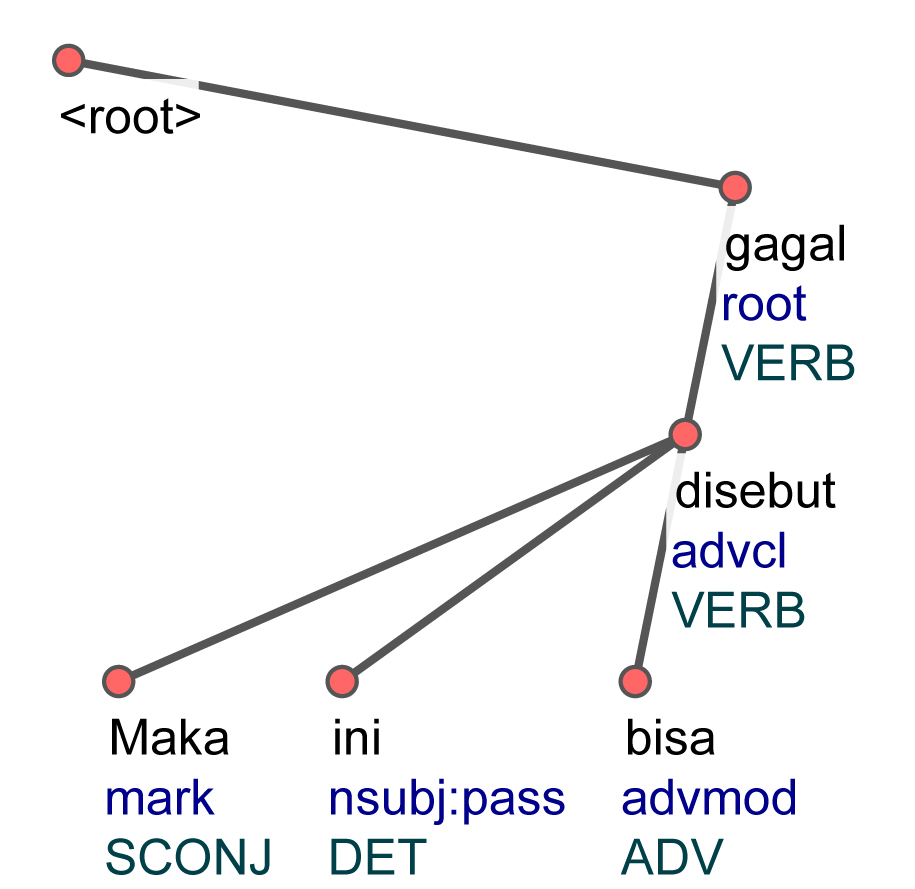
\includegraphics[width=0.35
	\textwidth] {pics/lampiran/lampiranls7359.jpg} 
	\caption{Bank pohon struktur dependensi ragam lisan dokumen 7359} 
	\label{fig:lampiranls7359} 
\end{figure}

\begin{figure}
	\centering 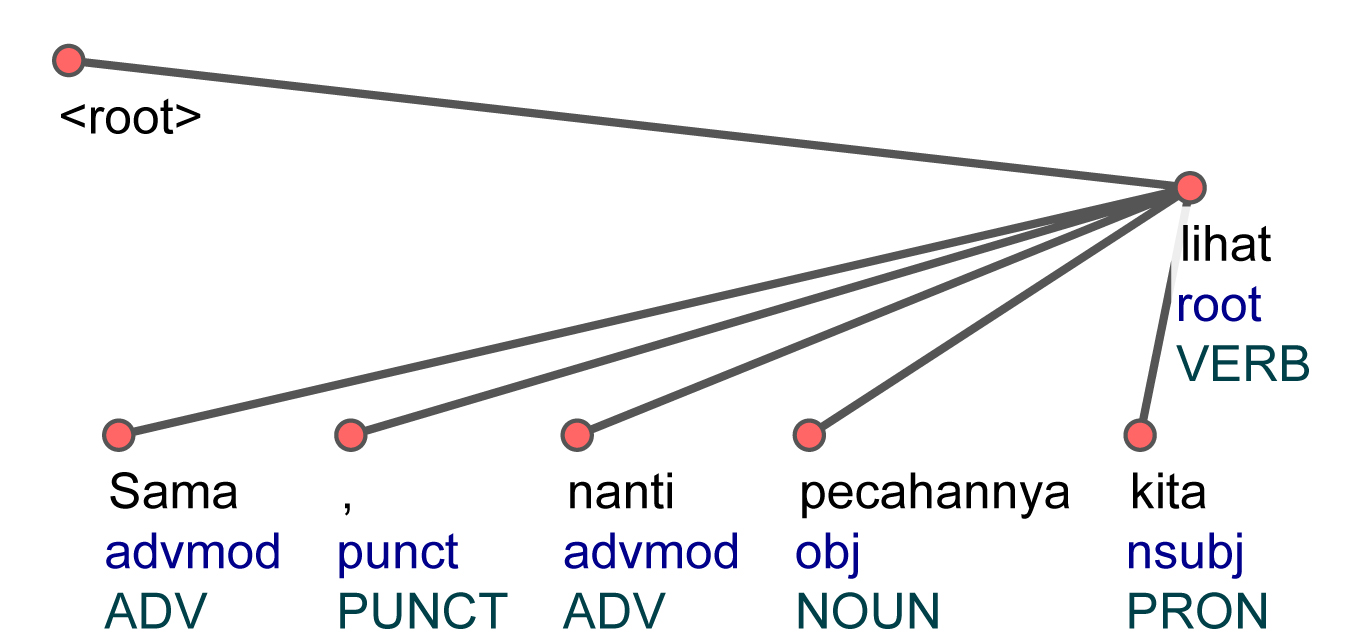
\includegraphics[width=0.5
	\textwidth] {pics/lampiran/lampiranls7375.jpg} 
	\caption{Bank pohon struktur dependensi ragam lisan dokumen 7375} 
	\label{fig:lampiranls7375} 
\end{figure}

